\documentclass{article}

\usepackage{arxiv}

\usepackage[utf8]{inputenc} % allow utf-8 input
\usepackage[T1]{fontenc}    % use 8-bit T1 fonts
\usepackage{lmodern}        % https://github.com/rstudio/rticles/issues/343
\usepackage{hyperref}       % hyperlinks
\usepackage{url}            % simple URL typesetting
\usepackage{booktabs}       % professional-quality tables
\usepackage{amsfonts}       % blackboard math symbols
\usepackage{nicefrac}       % compact symbols for 1/2, etc.
\usepackage{microtype}      % microtypography
\usepackage{graphicx}

\title{spmodel: Spatial Statistical Modeling and Prediction in
\textbf{R}}

\author{
    Michael Dumelle
    \thanks{Corresponding Author}
   \\
    United States \\
    Environmental Protection Agency \\
  200 SW 35th St, Corvallis, OR, 97333 \\
  \texttt{\href{mailto:Dumelle.Michael@epa.gov}{\nolinkurl{Dumelle.Michael@epa.gov}}} \\
   \And
    Matt Higham
   \\
    Department of Math, Computer Science, and Statistics \\
    St.~Lawrence University \\
  23 Romoda Drive, Canton, NY, 13617 \\
  \texttt{\href{mailto:mhigham@stlawu.edu}{\nolinkurl{mhigham@stlawu.edu}}} \\
   \And
    Jay M. Ver Hoef
   \\
    National Oceanic and Atmospheric Administration \\
    Alaska Fisheries Science Center \\
  Marine Mammal Laboratory, Seattle, WA, 98115 \\
  \texttt{\href{mailto:jay.verhoef@noaa.gov}{\nolinkurl{jay.verhoef@noaa.gov}}} \\
  }


% tightlist command for lists without linebreak
\providecommand{\tightlist}{%
  \setlength{\itemsep}{0pt}\setlength{\parskip}{0pt}}


% Pandoc citation processing
\newlength{\cslhangindent}
\setlength{\cslhangindent}{1.5em}
\newlength{\csllabelwidth}
\setlength{\csllabelwidth}{3em}
\newlength{\cslentryspacingunit} % times entry-spacing
\setlength{\cslentryspacingunit}{\parskip}
% for Pandoc 2.8 to 2.10.1
\newenvironment{cslreferences}%
  {}%
  {\par}
% For Pandoc 2.11+
\newenvironment{CSLReferences}[2] % #1 hanging-ident, #2 entry spacing
 {% don't indent paragraphs
  \setlength{\parindent}{0pt}
  % turn on hanging indent if param 1 is 1
  \ifodd #1
  \let\oldpar\par
  \def\par{\hangindent=\cslhangindent\oldpar}
  \fi
  % set entry spacing
  \setlength{\parskip}{#2\cslentryspacingunit}
 }%
 {}
\usepackage{calc}
\newcommand{\CSLBlock}[1]{#1\hfill\break}
\newcommand{\CSLLeftMargin}[1]{\parbox[t]{\csllabelwidth}{#1}}
\newcommand{\CSLRightInline}[1]{\parbox[t]{\linewidth - \csllabelwidth}{#1}\break}
\newcommand{\CSLIndent}[1]{\hspace{\cslhangindent}#1}

\usepackage{amsmath,amsfonts,amssymb}
\usepackage{bm, bbm}

\begin{document}
\maketitle


\begin{abstract}
\texttt{spmodel} is an \textbf{\textsf{R}} package used to fit,
summarize, and predict for a variety spatial statistical models.
Parameters are estimated using various methods. Additional modeling
features include anisotropy, random effects, partition factors, big data
approaches, and more. Model-fit statistics are used to summarize,
visualize, and compare models. Predictions at unobserved locations are
readily obtainable. This manuscript corresponds to \texttt{spmodel}
version 0.1.0.
\end{abstract}

\keywords{
    Spatial linear model
   \and
    Geostatistical model
   \and
    Autoregressive model
   \and
    Spatial Covariance
   \and
    Prediction (Kriging)
   \and
    Big Data
  }

\hypertarget{sec:introduction}{%
\section{Introduction}\label{sec:introduction}}

Spatial data are ubiquitous in everyday life and the scientific
literature. As such, it becoming is increasingly important to properly
analyze spatial data. Spatial data can be analyzed using a statistical
model that explicitly incorporates the spatial dependence among
observations. Incorporating this spatial dependence can be challenging,
but ignoring it often yields poor statistical models. \texttt{spmodel}
provides tools to easily incorporate this spatial dependence, building
upon commonly used \(\textbf{\textsf{R}}\) functions like \texttt{lm()}.

\texttt{spmodel} implements a model-based inference, which relies on
fitting a statistical model. This is a different way to analyze data
than design-based inference, which relies on random sampling and
estimators that incorporate the properties of the random sample. Spatial
random sampling and design-based inference can be performed using the
\texttt{spsurvey} \(\textbf{\textsf{R}}\) package (Dumelle, Kincaid, et
al. 2022). Though not explicitly required, random sampling can still
benefit model-based inference when analyzing spatial data (Dumelle,
Higham, et al. 2022).

Several \(\textbf{\textsf{R}}\) packages for analyzing point-referenced
(i.e., geostatistical) and areal (i.e., autoregressive) spatial data
from a model-based perspective exist. Data are point-referenced when
they are observed at point-locations indexed by x-coordinates and
y-coordinates on a spatially continuous surface with an infinite number
of locations. Data are areal they are observed as part of a finite
network of polygons whose connections are indexed by a neighborhood
structure. For example, the polygons may represent counties in a state
who are neighbors if they share at least one boundary. Existing
\(\textbf{\textsf{R}}\) packages for point-referenced data include
\texttt{fields} (Douglas Nychka et al. 2021), \texttt{FRK}
(Zammit-Mangion and Cressie 2021), \texttt{geoR} (Ribeiro Jr et al.
2022), \texttt{GpGp} (Guiness, Katzfuss, and Fahmy 2021), \texttt{gstat}
(E. J. Pebesma 2004), \texttt{LatticeKrig} (Nychka et al. 2016),
\texttt{spatial} (Venables and Ripley 2002), \texttt{spBayes} (Finley,
Banerjee, and Carlin 2007), and \texttt{spNNGP} (Finley, Datta, and
Banerjee 2022). Existing \(\textbf{\textsf{R}}\) packages for areal data
include and \texttt{CARBayes} (Lee 2013) and \texttt{hglm} (Ronnegard,
Shen, and Alam 2010). \texttt{spmodel} is capable of fitting statistical
models for both point-referenced and areal data and offers many features
missing from the aforementioned \(\textbf{\textsf{R}}\) packages.
Together in one \(\textbf{\textsf{R}}\) package, \texttt{spmodel} offers
detailed model summaries, extensive model diagnostics, random effects,
anisotropy, big data methods, prediction, and more.

The rest of this article is organized as follows. In
Section\(~\)\ref{sec:theomodel}, we give a brief theoretical
introduction to spatial linear models. In
Section\(~\)\ref{sec:modelfit}, we outline the variety of methods used
to estimate the parameters of spatial linear models. In
Section\(~\)\ref{sec:prediction}, we explain how to obtain predictions
at unobserved locations. In Section\(~\)\ref{sec:advfeatures}, we detail
some advanced modeling features, including random effects, partition
factors, anisotropy, and big data approaches. In
Section\(~\)\ref{sec:discussion}, we end with a short discussion. Before
proceeding, we load \texttt{spmodel} by running

\begin{verbatim}
R> library(spmodel)
\end{verbatim}

We will create visualizations using ggplot2 (Wickham 2016), which we
load by running

\begin{verbatim}
R> library(ggplot2)
\end{verbatim}

\hypertarget{sec:theomodel}{%
\section{The Spatial Linear Model}\label{sec:theomodel}}

Statistical linear models are often parameterized as
\begin{equation}\label{eq:lm}
 \mathbf{y} = \mathbf{X} \boldsymbol{\beta} + \boldsymbol{\epsilon},
\end{equation} where for a sample size \(n\), \(\mathbf{y}\) is an
\(n \times 1\) vector of response variables, \(\mathbf{X}\) is an
\(n \times p\) design (model) matrix of explanatory variables,
\(\boldsymbol{\beta}\) is an \(p \times 1\) vector of fixed effects
controlling the impact of \(\mathbf{X}\) on \(\mathbf{y}\), and
\(\boldsymbol{\epsilon}\) is an \(n \times 1\) vector of random errors.
Typically, it is assumed that
\(\text{E}(\boldsymbol{\epsilon}) = \mathbf{0}\) and
\(\text{Cov}(\boldsymbol{\epsilon}) = \sigma^2_\epsilon \mathbf{I}\),
where \(\text{E}(\cdot)\) denotes expectation, \(\text{Cov}(\cdot)\)
denotes covariance, \(\sigma^2_\epsilon\) denotes a variance parameter,
and \(\mathbf{I}\) denotes the identity matrix.

The model in Equation\(~\)\ref{eq:lm} assumes the elements of
\(\mathbf{y}\) are uncorrelated. Typically for spatial data, elements of
\(\mathbf{y}\) are correlated, as observations close together in space
tend to be more similar than observations far apart (Tobler 1970).
Failing to properly accommodate the spatial dependence in \(\mathbf{y}\)
can cause researchers to draw incorrect conclusions about their data. To
accommodate spatial dependence in \(\mathbf{y}\), an \(n \times 1\)
spatial random effect, \(\boldsymbol{\tau}\), is added to
Equation\(~\)\ref{eq:lm}, yielding the model
\begin{equation}\label{eq:splm}
 \mathbf{y} = \mathbf{X} \boldsymbol{\beta} + \boldsymbol{\tau} + \boldsymbol{\epsilon},
\end{equation} where \(\text{E}(\boldsymbol{\tau}) = \mathbf{0}\),
\(\text{Cov}(\boldsymbol{\tau}) = \sigma^2_\tau \mathbf{R}\), and
\(\mathbf{R}\) is a matrix that determines the spatial dependence
structure in \(\mathbf{y}\) and depends on a range parameter, \(\phi\).
The parameter \(\sigma^2_\tau\) is called the spatially dependent random
error variance or partial sill. The parameter \(\sigma^2_\epsilon\) is
called the spatially independent random error variance or nugget. These
two variance parameters are henceforth more intuitively written as
\(\sigma^2_{de}\) and \(\sigma^2_{ie}\), respectively. The covariance of
\(\mathbf{y}\) is denoted \(\boldsymbol{\Sigma}\) and given by
\(\sigma^2_{de} \mathbf{R} + \sigma^2_{ie} \mathbf{I}\). The parameters
that compose this covariance are typically referenced by the vector
\(\boldsymbol{\theta}\), which is called the covariance parameter
vector.

Equation\(~\)\ref{eq:splm} is called the spatial linear model. The
spatial linear model applies to both point-referenced and areal data.
The \texttt{splm()} function is used to fit spatial linear models for
point-referenced data (these are often called geostatistical models).
One spatial covariance function available in \texttt{splm()} is the
exponential spatial covariance function, which has an \(\mathbf{R}\)
matrix given by \begin{equation*}
  \mathbf{R} = \exp(-\mathbf{h} / \phi),
\end{equation*}\\
where \(\mathbf{h}\) is a matrix of Euclidean distances among
observations. Recall \(\phi\) is the range parameter, controlling the
behavior of \(\mathbf{R}\) as a function of distance. Parameterizations
for \texttt{splm()} spatial covariance types and their \(\mathbf{R}\)
matrices can be seen by running \texttt{help("splm",\ "spmodel")} or
\texttt{vignette("technical",\ "spmodel")}.

Data are areal when the elements in \(\mathbf{y}\) are observed as part
of a finite network of polygons whose connections are indexed by a
neighborhood structure. For example, the polygons may represent counties
in a state who are neighbors if they share at least one boundary. The
\texttt{spautor()} function is used to fit spatial linear models for
areal data (these are often called spatial autoregressive models). One
spatial autoregressive covariance function available in
\texttt{spautor()} is the simultaneous autoregressive spatial covariance
function, which has an \(\mathbf{R}\) matrix given by \begin{equation*}
  \mathbf{R} = [(\mathbf{I} - \phi \mathbf{W})(\mathbf{I} - \phi \mathbf{W})^\top]^{-1},
\end{equation*} where \(\mathbf{W}\) is a weight matrix describing the
neighborhood structure in \(\mathbf{y}\). Paremertizations for
\texttt{spautor()} spatial covariance types and their \(\mathbf{R}\)
matrices can be seen by running \texttt{help("spautor",\ "spmodel")} or
\texttt{vignette("technical",\ "spmodel")}.

\hypertarget{sec:modelfit}{%
\section{Model Fitting}\label{sec:modelfit}}

In this section, we show how to use the \texttt{splm()} and
\texttt{spautor()} functions to estimate parameters of the spatial
linear model. We also explore diagnostic tools in \texttt{spmodel} that
evaluate model fit. The \texttt{splm()} and \texttt{spautor()} functions
share similar syntactic structure with the \texttt{lm()} function used
to fit non-spatial linear models (linear models without spatial
dependence) from Equation\(~\)\ref{eq:lm}. \texttt{splm()} and
\texttt{spautor()} generally require at least three arguments:

\begin{itemize}
\tightlist
\item
  \texttt{formula}: a formula that describes the relationship between
  the response variable (\(\mathbf{y}\)) and explanatory variables
  (\(\mathbf{X}\))

  \begin{itemize}
  \tightlist
  \item
    \texttt{formula} in \texttt{splm()} is the same as \texttt{formula}
    in \texttt{lm()}
  \end{itemize}
\item
  \texttt{data}: a \texttt{data.frame} or \texttt{sf} object that
  contains the response variable, explanatory variables, and spatial
  information
\item
  \texttt{spcov\_type}: the spatial covariance type
  (\texttt{"exponential"}, \texttt{"matern"}, \texttt{"car"}, etc)
\end{itemize}

If \texttt{data} is an \texttt{sf} (E. Pebesma 2018) object, spatial
information is stored in the object's geometry. If \texttt{data} is a
\texttt{data.frame}, then for point-referenced data the x-coordinates
and y-coordinates must be provided via the \texttt{xcoord} and
\texttt{ycoord} arguments, and for areal data, the weight matrix must be
provided via the \texttt{W} argument. Appendix\(~\)\ref{app:caribou}
uses the \texttt{caribou} data, a \texttt{tibble} (a special
\texttt{data.frame}), to show how to explicitly provide spatial
information via \texttt{xcoord} and \texttt{ycoord} (in \texttt{splm()})
or \texttt{W} (in \texttt{spautor()}).

In the following subsections, we use the point-referenced \texttt{moss}
data, an \texttt{sf} object that contains data on heavy metals in mosses
near a mining road in Alaska. We view the first few rows of
\texttt{moss} by running

\begin{verbatim}
R> moss
\end{verbatim}

\begin{verbatim}
Simple feature collection with 365 features and 7 fields
Geometry type: POINT
Dimension:     XY
Bounding box:  xmin: -445884.1 ymin: 1929616 xmax: -383656.8 ymax: 2061414
Projected CRS: NAD83 / Alaska Albers
# A tibble: 365 x 8
   sample field_dup lab_rep year  sideroad log_dist2road log_Zn            geometry
   <fct>  <fct>     <fct>   <fct> <fct>            <dbl>  <dbl>         <POINT [m]>
 1 001PR  1         1       2001  N                 2.68   7.33 (-413585.3 1997623)
 2 001PR  1         2       2001  N                 2.68   7.38 (-413585.3 1997623)
 3 002PR  1         1       2001  N                 2.54   7.58 (-415367.2 1996769)
 4 003PR  1         1       2001  N                 2.97   7.63   (-417186 1995645)
 5 004PR  1         1       2001  N                 2.72   7.26 (-411756.6 1999907)
 6 005PR  1         1       2001  N                 2.76   7.65 (-419008.8 1994950)
 7 006PR  1         1       2001  S                 2.30   7.59 (-420822.6 1994480)
 8 007PR  1         1       2001  N                 2.78   7.16 (-404383.2 2007420)
 9 008PR  1         1       2001  N                 2.93   7.19 (-409964.1 2003323)
10 009PR  1         1       2001  N                 2.79   8.07 (-424469.7 1992184)
# ... with 355 more rows
\end{verbatim}

We can learn more about \texttt{moss} by running
\texttt{help("moss",\ "spmodel")}.

\hypertarget{estimation}{%
\subsection{Estimation}\label{estimation}}

Generally the covariance parameters (\(\boldsymbol{\theta}\)) and fixed
effects (\(\boldsymbol{\beta}\)) of the spatial linear model require
estimation. The default estimation method in \texttt{spmodel} is
restricted maximum likelihood (Patterson and Thompson 1971; Harville
1977; Wolfinger, Tobias, and Sall 1994). Maximum likelihood estimation
is also available. For point-referenced data, semivariogram weighted
least squares (Cressie 1985) and semivariogram composite likelihood
(Curriero and Lele 1999) are additional estimation methods. The
estimation method is controlled using the \texttt{estmethod} argument.

To visualize the distribution of log zinc concentration in the
\texttt{moss} data (Figure\(~\)\ref{fig:log_zn}), run

\begin{verbatim}
R> ggplot(moss, aes(color = log_Zn)) +
+   geom_sf(size = 2) +
+   scale_color_viridis_c() +
+   theme_gray(base_size = 14)
\end{verbatim}

\begin{figure}

{\centering 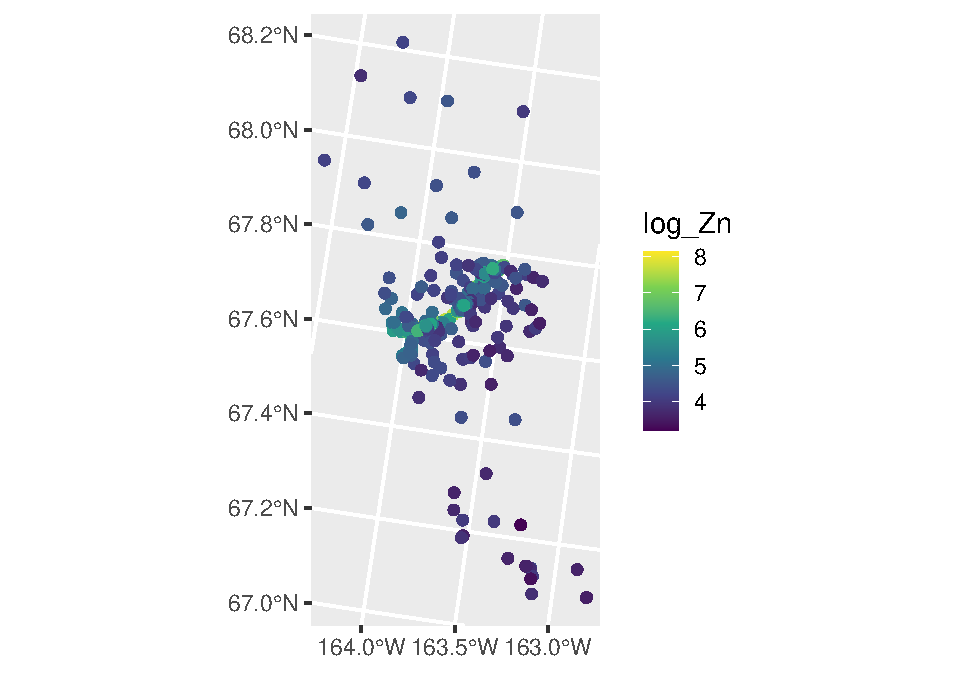
\includegraphics[width=0.65\linewidth]{preprint_files/figure-latex/log_zn-1} 

}

\caption{Distribution of log zinc concentration in the moss data.}\label{fig:log_zn}
\end{figure}

We estimate parameters of a spatial linear model regressing log zinc
concentration (\texttt{log\_Zn}) on log distance to a haul road
(\texttt{log\_dist2road}) using an exponential spatial covariance
function by running

\begin{verbatim}
R> spmod <- splm(log_Zn ~ log_dist2road, moss, spcov_type = "exponential")
\end{verbatim}

We summarize the model fit by running

\begin{verbatim}
R> summary(spmod)
\end{verbatim}

\begin{verbatim}
Call:
splm(formula = log_Zn ~ log_dist2road, data = moss, spcov_type = "exponential")

Residuals:
    Min      1Q  Median      3Q     Max 
-2.6801 -1.3606 -0.8103 -0.2485  1.1298 

Coefficients (fixed):
              Estimate Std. Error z value Pr(>|z|)    
(Intercept)    9.76825    0.25216   38.74   <2e-16 ***
log_dist2road -0.56287    0.02013  -27.96   <2e-16 ***
---
Signif. codes:  0 '***' 0.001 '**' 0.01 '*' 0.05 '.' 0.1 ' ' 1

Pseudo R-squared: 0.683

Coefficients ( spatial covariance):
       de        ie     range 
3.595e-01 7.897e-02 8.237e+03 
\end{verbatim}

The fixed effects coefficient table contains estimates, standard errors,
z-statistics, and asymptotic p-values for each fixed effect. From this
table, we notice there is evidence that log zinc concentration
significantly decreases with distance from the haul road (p-value
\textless{} 2e-16). We see the fixed effect estimates by running

\begin{verbatim}
R> coef(spmod)
\end{verbatim}

\begin{verbatim}
  (Intercept) log_dist2road 
    9.7682525    -0.5628713 
\end{verbatim}

The model summary also contains the exponential spatial covariance
parameter estimates, which we can view by running

\begin{verbatim}
R> coef(spmod, type = "spcov")
\end{verbatim}

\begin{verbatim}
          de           ie        range       rotate        scale 
3.595316e-01 7.896824e-02 8.236712e+03 0.000000e+00 1.000000e+00 
attr(,"class")
[1] "exponential"
\end{verbatim}

The dependent random error variance (\(\sigma^2_{de}\)) is estimated to
be approximately 0.36 and the independent random error variance
(\(\sigma^2_{ie}\)) is estimated to be approximately 0.079. The range
(\(\phi\)) is estimated to be approximately 8,237. The effective range
is the distance at which the spatial covariance is approximately zero.
For the exponential covariance, the effective range is \(3\phi\). This
means that observations whose distance is greater than 24,711 meters are
approximately uncorrelated. The \texttt{rotate} and \texttt{scale}
parameters affect the modeling of anisotropy
(Section\(~\)\ref{sec:anisotropy}). By default, they are assumed to be
zero and one, respectively, which means that anisotropy is not modeled
(i.e., the spatial covariance is assumed isotropic, or independent of
direction). We plot the fitted spatial covariance function
(Figure\(~\)\ref{fig:emp_spcov}) by running

\begin{verbatim}
R> plot(spmod, which = 7)
\end{verbatim}

\begin{figure}

{\centering 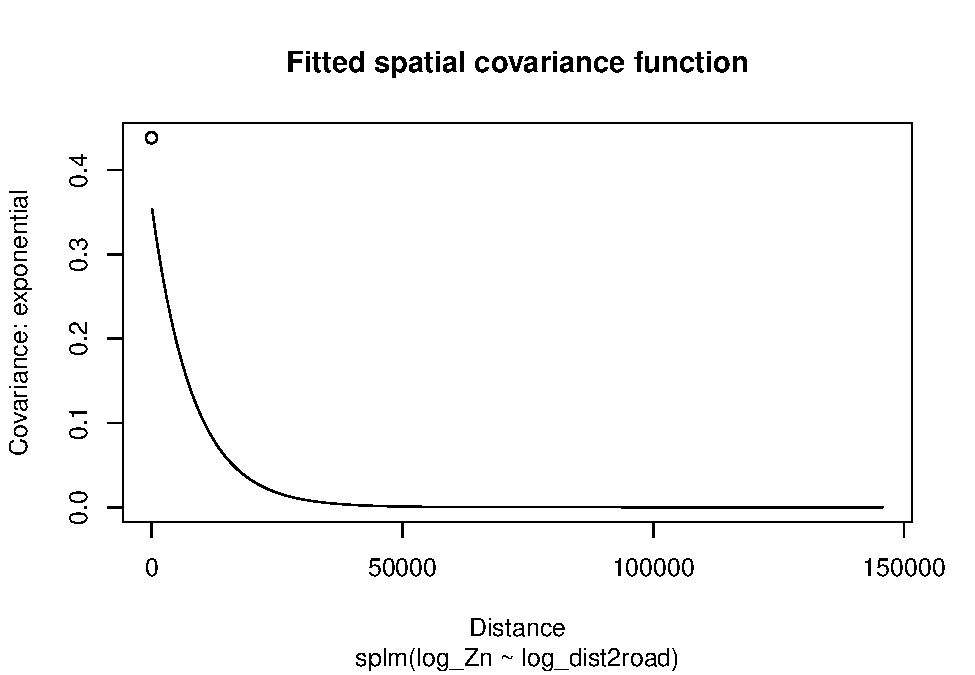
\includegraphics[width=0.75\linewidth]{preprint_files/figure-latex/emp_spcov-1} 

}

\caption{Empirical spatial covariance of fitted model.}\label{fig:emp_spcov}
\end{figure}

We can learn more about the plots available for fitted models by running
\texttt{help("plot.spmod",\ "spmodel")}.

\hypertarget{model-fit-statistics}{%
\subsection{Model-Fit Statistics}\label{model-fit-statistics}}

The quality of model fit can be assessed using a variety of statistics
readily available in \texttt{spmodel}. The first model-fit statistic we
consider is the pseudo R-squared. The pseudo R-squared is a
generalization of the classical R-squared from non-spatial linear models
that quantifies the proportion of variability in the data explained by
the fixed effects. The pseudo R-squared is defined as \begin{equation*}
PR2 = 1 - \frac{\mathcal{D}(\boldsymbol{\hat{\Theta}})}{\mathcal{D}(\boldsymbol{\hat{\Theta}}_0)},
\end{equation*} where \(\mathcal{D}(\boldsymbol{\hat{\Theta}})\) is the
deviance of the fitted model indexed by parameter vector
\(\boldsymbol{\hat{\Theta}}\) and
\(\mathcal{D}(\boldsymbol{\hat{\Theta}}_0)\) is the deviance of an
intercept-only model indexed by parameter vector
\(\boldsymbol{\hat{\Theta}}_0\). We compute the pseudo R-squared by
running

\begin{verbatim}
R> pseudoR2(spmod)
\end{verbatim}

\begin{verbatim}
[1] 0.6829687
\end{verbatim}

Roughly 68\% of the variability in log zinc is explained by log distance
from the road. The pseudo R-squared can be adjusted to account for the
number of explanatory variables using the \texttt{adjust} argument.
Pseudo R-squared (and the adjusted version) is most helpful for
comparing models that have the same covariance structure.

The next two model-fit statistics we consider are the spatial AIC and
AICc (Hoeting et al. 2006). The AIC and AICc evaluate the fit of a model
with a penalty for the number of parameters estimated. This penalty
balances model fit and model parsimony. The AICc is a correction to AIC
for small sample sizes. As the sample size increases, the AIC and AICc
become closer to one another. The lower the AIC and AICc, the better the
balance of model fit and parsimony.

The spatial AIC and AICc are given by \begin{equation*}\label{eq:sp_aic}
  \begin{split}
    \text{AIC} & = -2\ell(\hat{\boldsymbol{\Theta}}) + 2(|\hat{\boldsymbol{\Theta}}|) \\
    \text{AICc} & = -2\ell(\hat{\boldsymbol{\Theta}}) + 2n(|\hat{\boldsymbol{\Theta}}|) / (n - |\hat{\boldsymbol{\Theta}}| - 1),
  \end{split}
\end{equation*} where \(\ell(\hat{\boldsymbol{\Theta}})\) is the
log-likelihood of the data evaluated at the estimated parameter vector
\(\hat{\boldsymbol{\Theta}}\) maximizing \(\ell(\boldsymbol{\Theta})\),
and \(n\) is the sample size. For maximum likelihood,
\(\hat{\boldsymbol{\Theta}} = \{\hat{\boldsymbol{\theta}}, \hat{\boldsymbol{\beta}}\}\).
For restricted maximum likelihood
\(\hat{\boldsymbol{\Theta}} = \{\hat{\boldsymbol{\theta}}\}\). AIC
comparisons between a model fit using restricted maximum likelihood and
a model fit using maximum likelihood are meaningless, as the models are
fit with different likelihoods. AIC comparisons between models fit using
restricted maximum likelihood are only valid when the models have the
same fixed effect structure. In contrast, AIC comparisons between models
fit using maximum likelihood are valid when the models have different
fixed effect structures.

Suppose we want to quantify the difference in model quality between the
spatial model and a non-spatial model using the AIC and AICc criteria.
We fit a non-spatial model (Equation\(~\)\ref{eq:lm}) in
\texttt{spmodel} by running

\begin{verbatim}
R> lmod <- splm(log_Zn ~ log_dist2road, moss, spcov_type = "none")
\end{verbatim}

We compute the spatial AIC and AICc of the spatial model and non-spatial
model by running

\begin{verbatim}
R> AIC(spmod, lmod)
\end{verbatim}

\begin{verbatim}
      df      AIC
spmod  3 373.2089
lmod   1 636.0635
\end{verbatim}

\begin{verbatim}
R> AICc(spmod, lmod)
\end{verbatim}

\begin{verbatim}
      df     AICc
spmod  3 373.2754
lmod   1 636.0745
\end{verbatim}

The noticeably lower AIC and AICc of of the spatial model indicate that
it is a better fit to the data than the non-spatial model.

Another approach to comparing the model fits is to perform leave-one-out
cross validation. In leave-one-out cross validation, a single
observation is removed from the data, the model is re-fit, and a
prediction is made for the held-out observation. Then a loss metric like
mean-squared-prediction error is computed and used to evaluate model
fit. The lower the mean-squared-prediction error, the better the model
fit. For computational efficiency, leave-one-out cross validation in
\texttt{spmodel} is performed by first estimating
\(\boldsymbol{\theta}\) using all the data and then re-estimating
\(\boldsymbol{\beta}\) for each observation. We perform leave-one-out
cross validation for the spatial and non-spatial model by running

\begin{verbatim}
R> loocv(spmod)
\end{verbatim}

\begin{verbatim}
[1] 0.1110895
\end{verbatim}

\begin{verbatim}
R> loocv(lmod)
\end{verbatim}

\begin{verbatim}
[1] 0.3237897
\end{verbatim}

The noticeably lower mean-squared-prediction error of the spatial model
indicates that it is a better fit to the data than the non-spatial
model.

\hypertarget{diagnostics}{%
\subsection{Diagnostics}\label{diagnostics}}

An observation is said to have high leverage if its combination of
explanatory variable values is far from the mean vector of the
explanatory variables. For a non-spatial model, the leverage of the
\(i\)th observation is the \(i\)th diagonal element of the hat matrix
given by \begin{equation*}
  \mathbf{H} = \mathbf{X}(\mathbf{X}^\top\mathbf{X})^{-1}\mathbf{X}^\top .
\end{equation*} For a spatial model, the leverage of the \(i\)th
observation is the \(i\)th diagonal element of the spatial hat matrix
given by \begin{equation*}
  \mathbf{H}^* = (\mathbf{X}^* (\mathbf{X}^{* \top} \mathbf{X})^{-1} \mathbf{X}^{* \top}) ,
\end{equation*} where
\(\mathbf{X}^* = \boldsymbol{\Sigma}^{-1/2}\mathbf{X}\) and
\(\boldsymbol{\Sigma}^{-1/2}\) is the matrix square root of the
covariance matrix, \(\boldsymbol{\Sigma}\) (Montgomery, Peck, and Vining
2021). The spatial hat matrix can be viewed as the non-spatial hat
matrix applied to the ``whitened'' \(\mathbf{X}\) matrix,
\(\mathbf{X}^*\). We compute the hat values (leverage) by running

\begin{verbatim}
R> hatvalues(spmod)
\end{verbatim}

The larger the hat value, the larger the leverage.

The fitted value of an observation is the estimated mean response given
the observation's explanatory variable values and the model fit:
\begin{equation*}
  \hat{\mathbf{y}} = \mathbf{X} \hat{\boldsymbol{\beta}}.
\end{equation*} We compute the fitted values by running

\begin{verbatim}
R> fitted(spmod)
\end{verbatim}

Fitted values for the spatially dependent random errors
(\(\boldsymbol{\tau}\)), spatially independent random errors
(\(\boldsymbol{\epsilon}\)), and random effects can also be obtained via
\texttt{fitted()} by changing the \texttt{type} argument.

The residuals act as estimates of errors, measuring each response's
deviation from its fitted value. The raw residuals are given by
\begin{equation*}
  \mathbf{e}_{r} = \mathbf{y} - \hat{\mathbf{y}}.
\end{equation*} We compute the raw residuals of the spatial model by
running

\begin{verbatim}
R> residuals(spmod)
\end{verbatim}

The raw residuals are typically not directly checked for linear model
assumptions, as they have covariance closely resembling the covariance
of \(\mathbf{y}\). These residuals can be ``whitened'' by
pre-multiplying by \(\boldsymbol{\hat{\Sigma}}^{-1/2}\), yielding the
Pearson residuals: \begin{equation*}
  \mathbf{e}_{p} = \boldsymbol{\hat{\Sigma}}^{-1/2}\mathbf{e}_{r}.
\end{equation*} When the model is correct, the Pearson residuals have
mean zero, variance approximately one, and are uncorrelated. We compute
the Pearson residuals of the spatial model by running

\begin{verbatim}
R> residuals(spmod, type = "pearson")
\end{verbatim}

The covariance of \(\mathbf{e}_{p}\) is \((\mathbf{I} - \mathbf{H}^*)\),
which is approximately \(\mathbf{I}\) for large sample sizes. Explicitly
dividing \(\mathbf{e}_{p}\) by the respective diagonal element of
\((\mathbf{I} - \mathbf{H}^*)\) yields the standardized residuals:
\begin{equation*}
  \mathbf{e}_{s} = \frac{\mathbf{e}_{p}}{\sqrt{(1 - diag(\mathbf{H}^*))}},
\end{equation*} where \(diag(\mathbf{H}^*)\) denotes the diagonal of
\(\mathbf{H}^*\).

We compute the standardized residuals of the spatial model by running

\begin{verbatim}
R> residuals(spmod, type = "standardized")
\end{verbatim}

or

\begin{verbatim}
R> rstandard(spmod)
\end{verbatim}

When the model is correct, the standardized residuals have mean zero,
variance one, and are uncorrelated. It is common to check linear model
assumptions through visualizations. We can plot the standardized
residuals vs fitted values by running

\begin{verbatim}
R> plot(spmod, which = 1) # figure omitted
\end{verbatim}

When the model is correct, the standardized residuals should be evenly
spread around zero with no discernible pattern. We can plot a normal
QQ-plot of the standardized residuals by running

\begin{verbatim}
R> plot(spmod, which = 2) # figure omitted
\end{verbatim}

When the standardized residuals are normally distributed, they should
closely follow the normal QQ-line.

An observation is said to be influential if its omission has a large
impact on model fit. Typically this is measured using Cook's distance
(Cook and Weisberg 1982). For the non-spatial model, the Cook's distance
of the \(i\)th observation is denoted \(\mathbf{D}\) and given by
\begin{equation*}
  \mathbf{D} = \mathbf{e}_{s}^2 \frac{diag(\mathbf{H})}{p(1 - diag(\mathbf{H}))} .
\end{equation*} For a spatial model, the Cook's distance of the \(i\)th
observation is denoted \(\mathbf{D}^*\) and given by \begin{equation*}
  \mathbf{D}^* = \mathbf{e}_{s}^2 \frac{diag(\mathbf{H}^*)}{p(1 - diag(\mathbf{H}^*))} .
\end{equation*} The larger the Cook's distance, the larger the
influence. We compute Cook's distance by running

\begin{verbatim}
R> cooks.distance(spmod)
\end{verbatim}

We visualize the Cook's distance versus leverage (hat values) by running

\begin{verbatim}
R> plot(spmod, which = 6) # figure omitted
\end{verbatim}

\hypertarget{the-broom-functions-tidy-glance-and-augment}{%
\subsection{\texorpdfstring{The broom functions: \texttt{tidy()},
\texttt{glance()}, and
\texttt{augment()}}{The broom functions: tidy(), glance(), and augment()}}\label{the-broom-functions-tidy-glance-and-augment}}

The \texttt{tidy()}, \texttt{glance()}, and \texttt{augment()} functions
from the broom \textbf{\textsf{R}} package (Robinson, Hayes, and Couch
2021) are defined for \texttt{spmodel} objects. The \texttt{tidy()}
function returns a tidy tibble of the coefficient table from
\texttt{summary()}:

\begin{verbatim}
R> tidy(spmod)
\end{verbatim}

\begin{verbatim}
# A tibble: 2 x 5
  term          estimate std.error statistic p.value
  <chr>            <dbl>     <dbl>     <dbl>   <dbl>
1 (Intercept)      9.77     0.252       38.7       0
2 log_dist2road   -0.563    0.0201     -28.0       0
\end{verbatim}

This tibble format makes it easy to pull out the coefficient names,
estimates, standard errors, z-statistics, and p-values from the
\texttt{summary()} output. The \texttt{glance()} function returns a tidy
tibble of model-fit statistics:

\begin{verbatim}
R> glance(spmod)
\end{verbatim}

\begin{verbatim}
# A tibble: 1 x 9
      n     p  npar value   AIC  AICc logLik deviance pseudo.r.squared
  <int> <dbl> <int> <dbl> <dbl> <dbl>  <dbl>    <dbl>            <dbl>
1   365     2     3  367.  373.  373.  -184.      363            0.683
\end{verbatim}

The \texttt{glances()} function can be used to look at many models
simultaneously:

\begin{verbatim}
R> glances(spmod, lmod)
\end{verbatim}

\begin{verbatim}
# A tibble: 2 x 10
  model     n     p  npar value   AIC  AICc logLik deviance pseudo.r.squared
  <chr> <int> <dbl> <int> <dbl> <dbl> <dbl>  <dbl>    <dbl>            <dbl>
1 spmod   365     2     3  367.  373.  373.  -184.     363             0.683
2 lmod    365     2     1  634.  636.  636.  -317.     363.            0.671
\end{verbatim}

The \texttt{augment()} function augments the original data with model
diagnostics:

\begin{verbatim}
R> augment(spmod)
\end{verbatim}

\begin{verbatim}
Simple feature collection with 365 features and 7 fields
Geometry type: POINT
Dimension:     XY
Bounding box:  xmin: -445884.1 ymin: 1929616 xmax: -383656.8 ymax: 2061414
Projected CRS: NAD83 / Alaska Albers
# A tibble: 365 x 8
   log_Zn log_dist2road .fitted .resid    .hat  .cooksd .std.resid
 *  <dbl>         <dbl>   <dbl>  <dbl>   <dbl>    <dbl>      <dbl>
 1   7.33          2.68    8.26 -0.928 0.102   0.112        -1.48 
 2   7.38          2.68    8.26 -0.880 0.0101  0.000507     -0.316
 3   7.58          2.54    8.34 -0.755 0.0170  0.000475     -0.236
 4   7.63          2.97    8.09 -0.464 0.0137  0.000219      0.178
 5   7.26          2.72    8.24 -0.977 0.0177  0.00515      -0.762
 6   7.65          2.76    8.21 -0.568 0.0147  0.000929     -0.355
 7   7.59          2.30    8.47 -0.886 0.0170  0.00802      -0.971
 8   7.16          2.78    8.20 -1.05  0.0593  0.0492       -1.29 
 9   7.19          2.93    8.12 -0.926 0.00793 0.000451     -0.337
10   8.07          2.79    8.20 -0.123 0.0265  0.00396       0.547
# ... with 355 more rows, and 1 more variable: geometry <POINT [m]>
\end{verbatim}

By default, only the columns of \texttt{data} used to fit the model are
returned alongside the diagnostics. All original columns of
\texttt{data} are returned by setting \texttt{drop} to \texttt{FALSE}.

\hypertarget{an-areal-data-example}{%
\subsection{An Areal Data Example}\label{an-areal-data-example}}

Next we use the areal \texttt{seal} data, an \texttt{sf} object that
contains the log of the estimated harbor-seal trends from abundance data
across polygons in Alaska. We view the first few rows of \texttt{seal}
by running

\begin{verbatim}
R> seal
\end{verbatim}

\begin{verbatim}
Simple feature collection with 62 features and 1 field
Geometry type: POLYGON
Dimension:     XY
Bounding box:  xmin: 913618.8 ymin: 1007542 xmax: 1116002 ymax: 1145054
Projected CRS: NAD83 / Alaska Albers
# A tibble: 62 x 2
   log_trend                                                                      geometry
       <dbl>                                                                 <POLYGON [m]>
 1  NA       ((1035002 1054710, 1035002 1054542, 1035002 1053542, 1035002 1052542, 103500~
 2  -0.282   ((1037002 1039492, 1037006 1039490, 1037017 1039492, 1037035 1039496, 103704~
 3  -0.00121 ((1070158 1030216, 1070185 1030207, 1070187 1030207, 1070211 1030207, 107027~
 4   0.0354  ((1054906 1034826, 1054931 1034821, 1054936 1034822, 1055001 1034828, 105500~
 5  -0.0160  ((1025142 1056940, 1025184 1056889, 1025222 1056836, 1025256 1056780, 102527~
 6   0.0872  ((1026035 1044623, 1026037 1044605, 1026072 1044610, 1026083 1044612, 102611~
 7  -0.266   ((1100345 1060709, 1100287 1060706, 1100228 1060706, 1100170 1060711, 110011~
 8   0.0743  ((1030247 1029637, 1030248 1029637, 1030265 1029642, 1030328 1029656, 103039~
 9  NA       ((1043093 1020553, 1043097 1020550, 1043101 1020550, 1043166 1020557, 104323~
10  -0.00961 ((1116002 1024542, 1116002 1023542, 1116002 1022542, 1116002 1021554, 111598~
# ... with 52 more rows
\end{verbatim}

We can learn more about the data by running
\texttt{help("seal",\ "spmodel")}.

To visualize the distribution of log seal trends in the \texttt{seal}
data (Figure\(~\)\ref{fig:log_trend}), run

\begin{verbatim}
R> ggplot(seal, aes(fill = log_trend)) +
+   geom_sf(size = 0.75) +
+   scale_fill_viridis_c() +
+   theme_gray(base_size = 14)
\end{verbatim}

\begin{figure}

{\centering 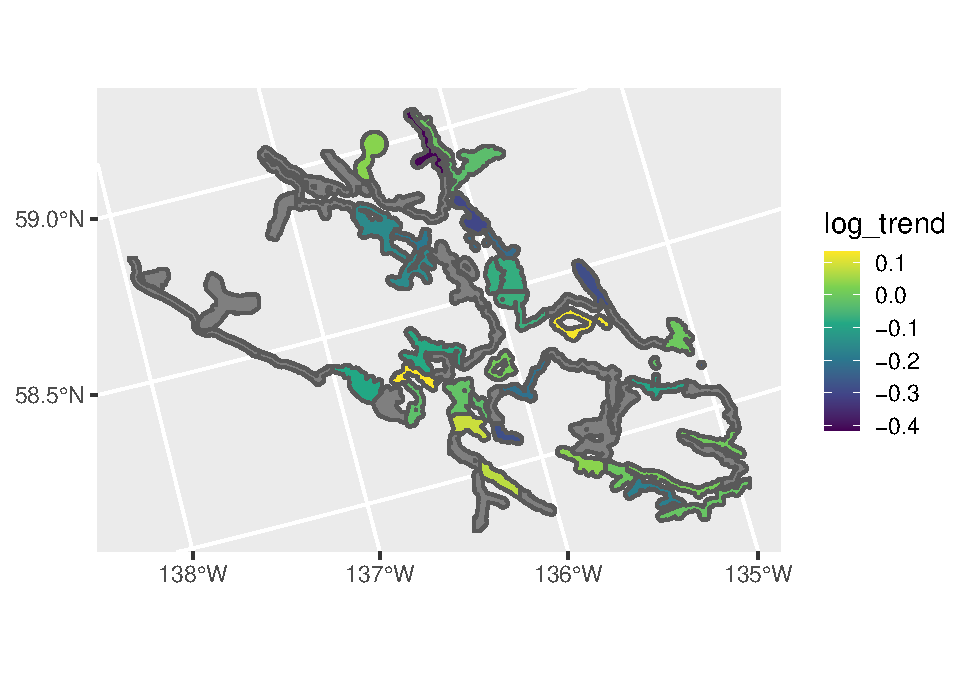
\includegraphics[width=0.65\linewidth]{preprint_files/figure-latex/log_trend-1} 

}

\caption{Distribution of log seal trends in the seal data. Polygons are gray where seal trends were not available.}\label{fig:log_trend}
\end{figure}

Polygons are considered neighbors if they share at least one boundary.
Polygons are gray if the log trend is missing. It is important to keep
these missing observations in the data while fitting the model to
preserve the neighborhood structure.

We estimate parameters of a spatial autoregressive model regressing log
seal trends (\texttt{log\_trend}) on an intercept using a conditional
autoregressive (CAR) spatial covariance by running

\begin{verbatim}
R> sealmod <- spautor(log_trend ~ 1, seal, spcov_type = "car")
\end{verbatim}

By default, \texttt{spautor()} calculates the weight matrix internally
by defining observations as neighbors if they share at least one border
(observations are not neighbors with themselves), uses row
standardization, and assumes \texttt{ie} equals zero.

We tidy and glance at the fitted model and augment the data by running

\begin{verbatim}
R> tidy(sealmod)
\end{verbatim}

\begin{verbatim}
# A tibble: 1 x 5
  term        estimate std.error statistic p.value
  <chr>          <dbl>     <dbl>     <dbl>   <dbl>
1 (Intercept)  -0.0710    0.0250     -2.85 0.00443
\end{verbatim}

\begin{verbatim}
R> glance(sealmod)
\end{verbatim}

\begin{verbatim}
# A tibble: 1 x 9
      n     p  npar value   AIC  AICc logLik deviance pseudo.r.squared
  <int> <dbl> <int> <dbl> <dbl> <dbl>  <dbl>    <dbl>            <dbl>
1    34     1     3 -36.9 -30.9 -30.1   18.4     32.9                0
\end{verbatim}

\begin{verbatim}
R> augment(sealmod)
\end{verbatim}

\begin{verbatim}
Simple feature collection with 34 features and 6 fields
Geometry type: POLYGON
Dimension:     XY
Bounding box:  xmin: 980001.5 ymin: 1010815 xmax: 1116002 ymax: 1145054
Projected CRS: NAD83 / Alaska Albers
# A tibble: 34 x 7
   log_trend .fitted  .resid   .hat .cooksd .std.resid                            geometry
 *     <dbl>   <dbl>   <dbl>  <dbl>   <dbl>      <dbl>                       <POLYGON [m]>
 1  -0.282   -0.0710 -0.211  0.0179 0.0233      -1.14  ((1037002 1039492, 1037006 1039490~
 2  -0.00121 -0.0710  0.0698 0.0699 0.0412       0.767 ((1070158 1030216, 1070185 1030207~
 3   0.0354  -0.0710  0.106  0.0218 0.0109       0.705 ((1054906 1034826, 1054931 1034821~
 4  -0.0160  -0.0710  0.0550 0.0343 0.00633      0.430 ((1025142 1056940, 1025184 1056889~
 5   0.0872  -0.0710  0.158  0.0229 0.0299       1.14  ((1026035 1044623, 1026037 1044605~
 6  -0.266   -0.0710 -0.195  0.0280 0.0493      -1.33  ((1100345 1060709, 1100287 1060706~
 7   0.0743  -0.0710  0.145  0.0480 0.0818       1.30  ((1030247 1029637, 1030248 1029637~
 8  -0.00961 -0.0710  0.0614 0.0143 0.00123      0.293 ((1116002 1024542, 1116002 1023542~
 9  -0.182   -0.0710 -0.111  0.0131 0.0155      -1.09  ((1079864 1025088, 1079895 1025084~
10   0.00351 -0.0710  0.0745 0.0340 0.0107       0.561 ((1110363 1037056, 1110346 1037040~
# ... with 24 more rows
\end{verbatim}

\hypertarget{sec:prediction}{%
\section{Prediction}\label{sec:prediction}}

In this section, we show how to use \texttt{predict()} to perform
spatial prediction (also called Kriging) in \texttt{spmodel}. We fit a
model using the point-referenced \texttt{sulfate} data, an \texttt{sf}
object that contains sulfate measurements in the conterminous United
States. We make predictions for each location in the point-referenced
\texttt{sulfate\_preds} data, an \texttt{sf} object that contains
locations in the conterminous United States at which to predict sulfate.
We visualize the distribution of the sulfate data
(Figure\(~\)\ref{fig:sulfate}, left) by running

\begin{verbatim}
R> ggplot(sulfate, aes(color = sulfate)) +
+   geom_sf(size = 2.5) +
+   scale_color_viridis_c(limits = c(0, 45)) +
+   theme_gray(base_size = 18)
\end{verbatim}

We fit a spatial linear model regressing sulfate on an intercept using a
spherical spatial covariance function by running

\begin{verbatim}
R> sulfmod <- splm(sulfate ~ 1, sulfate, spcov_type = "spherical")
\end{verbatim}

Then we obtain best linear unbiased predictions (Kriging predictions)
using \texttt{predict()}, where the \texttt{newdata} argument contains
the locations at which to predict:

\begin{verbatim}
R> predict(sulfmod, newdata = sulfate_preds)
\end{verbatim}

We make and predictions at the locations in \texttt{sulfate\_preds} and
store them as a new variable called \texttt{preds} in the
\texttt{sulfate\_preds} data set and then visualize them
(Figure\(~\)\ref{fig:sulfate}, right) by running

\begin{verbatim}
R> sulfate_preds$preds <- predict(sulfmod, newdata = sulfate_preds)
R> ggplot(sulfate_preds, aes(color = preds)) +
+   geom_sf(size = 2.5) +
+   scale_color_viridis_c(limits = c(0, 45)) +
+   theme_gray(base_size = 18)
\end{verbatim}

\begin{figure}

{\centering 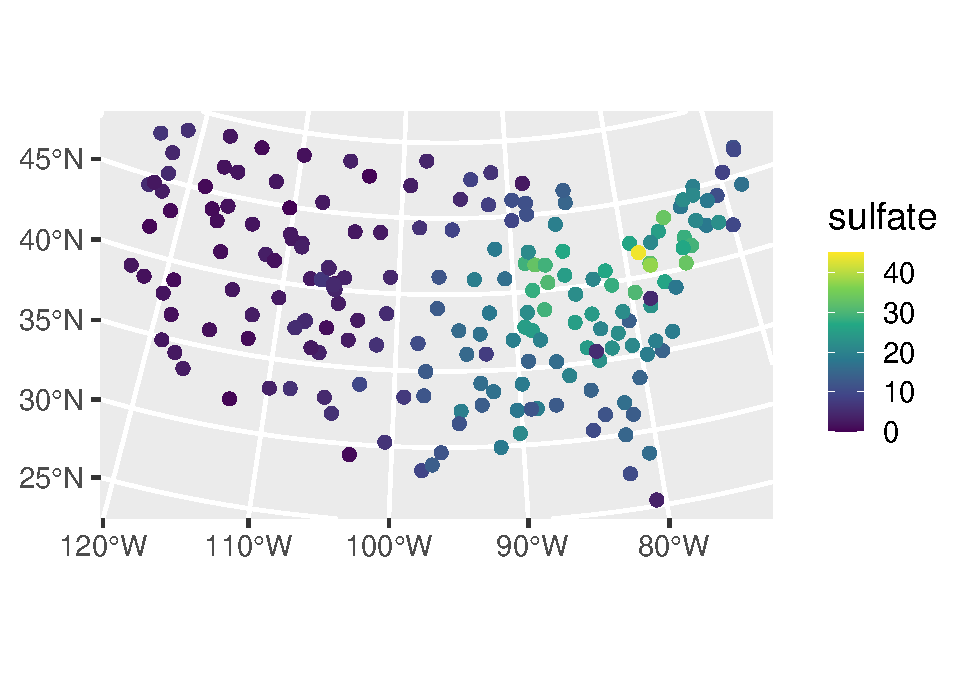
\includegraphics[width=0.49\linewidth]{preprint_files/figure-latex/sulfate-1} 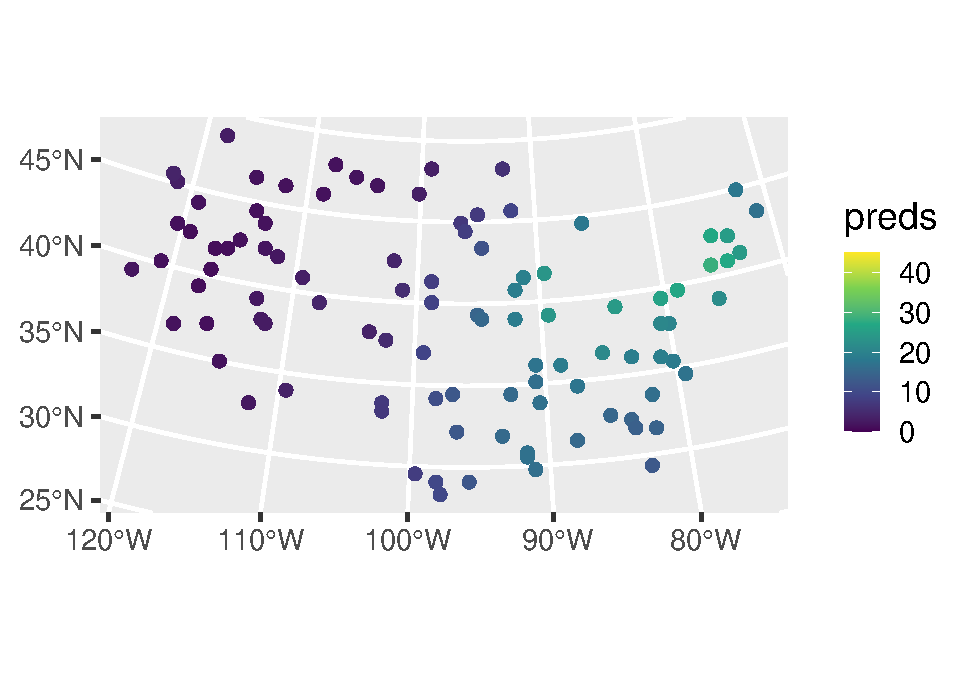
\includegraphics[width=0.49\linewidth]{preprint_files/figure-latex/sulfate-2} 

}

\caption{Distribution of observed sulfate (left) and sulfate predictions (right) in the conterminous United States.}\label{fig:sulfate}
\end{figure}

If explanatory variables were used to fit the model, the same
explanatory variables must be included in \texttt{newdata} with the same
names they have in \texttt{data}. If \texttt{data} is a
\texttt{data.frame}, coordinates must be included in \texttt{newdata}
with the same names as they have in \texttt{data}. If \texttt{data} is
an \texttt{sf} object, coordinates must be included in \texttt{newdata}
with the same geometry name as they have in \texttt{data}. When using
projected coordinates, the projection for \texttt{newdata} should be the
same as the projection for \texttt{data}.

Prediction standard errors are returned by setting the \texttt{se.fit}
argument to \texttt{TRUE}:

\begin{verbatim}
R> predict(sulfmod, newdata = sulfate_preds, se.fit = TRUE)
\end{verbatim}

The \texttt{interval} argument determines the type of interval returned.
If \texttt{interval} is \texttt{"none"} (the default), no interval is
returned. If \texttt{interval} is \texttt{"prediction"}, a
\texttt{100\ *\ level}\% prediction interval is returned (the default is
a 95\% prediction interval):

\begin{verbatim}
R> predict(sulfmod, newdata = sulfate_preds, interval = "prediction")
\end{verbatim}

If \texttt{interval} is \texttt{"confidence"}, the predictions are
instead the estimated mean given each observation's explanatory variable
values. The corresponding \texttt{100\ *\ level}\% confidence interval
is returned:

\begin{verbatim}
R> predict(sulfmod, newdata = sulfate_preds, interval = "confidence")
\end{verbatim}

Previously we used the \texttt{augment()} function to augment
\texttt{data} with model diagnostics. We can also use \texttt{augment()}
to augment \texttt{newdata} with predictions, standard errors, and
intervals. We remove the model predictions from \texttt{sulfate\_preds}
before showing how \texttt{augment()} is used to obtain the same
predictions by running

\begin{verbatim}
R> sulfate_preds$preds <- NULL
\end{verbatim}

We then view the first few rows of \texttt{sulfate\_preds} augmented
with a 90\% prediction interval by running

\begin{verbatim}
R> augment(sulfmod, newdata = sulfate_preds, interval = "prediction", level = 0.90)
\end{verbatim}

\begin{verbatim}
Simple feature collection with 100 features and 3 fields
Geometry type: POINT
Dimension:     XY
Bounding box:  xmin: -2283774 ymin: 582930.5 xmax: 1985906 ymax: 3037173
Projected CRS: NAD83 / Conus Albers
# A tibble: 100 x 4
   .fitted .lower .upper            geometry
 *   <dbl>  <dbl>  <dbl>         <POINT [m]>
 1    1.40  -5.33   8.14  (-1771413 1752976)
 2   24.5   18.2   30.8    (1018112 1867127)
 3    8.99   2.36  15.6  (-291256.8 1553212)
 4   16.4    9.92  23.0    (1274293 1267835)
 5    4.91  -1.56  11.4  (-547437.6 1638825)
 6   26.7   20.4   33.0    (1445080 1981278)
 7    3.00  -3.65   9.66  (-1629090 3037173)
 8   14.3    7.97  20.6    (1302757 1039534)
 9    1.49  -5.08   8.06  (-1429838 2523494)
10   14.4    7.97  20.8    (1131970 1096609)
# ... with 90 more rows
\end{verbatim}

Here \texttt{.fitted} represents the predictions.

Alternatively, we can include missing responses (\texttt{NA} values) in
the data used for model fitting. The missing responses will be ignored
for model fitting but stored in the fitted model object. We can add a
column of missing responses to \texttt{sulfate\_preds}, bind it together
with \texttt{sulfate}, and re-fit the model by running

\begin{verbatim}
R> sulfate_preds$sulfate <- NA
R> sulfate_with_NA <- rbind(sulfate, sulfate_preds)
R> sulfmod_with_NA <- splm(sulfate ~ 1, sulfate_with_NA, "spherical")
\end{verbatim}

We can then make predictions at the observations with missing responses
by running

\begin{verbatim}
R> predict(sulfmod_with_NA)
\end{verbatim}

This call to \texttt{predict()} finds in \texttt{sulfmod\_with\_NA} the
\texttt{newdata} object, which is a subset of \texttt{data} that
contains only the observations with missing responses:

\begin{verbatim}
R> sulfmod_with_NA$newdata
\end{verbatim}

\begin{verbatim}
Simple feature collection with 100 features and 1 field
Geometry type: POINT
Dimension:     XY
Bounding box:  xmin: -2283774 ymin: 582930.5 xmax: 1985906 ymax: 3037173
Projected CRS: NAD83 / Conus Albers
First 10 features:
    sulfate                  geometry
198      NA  POINT (-1771413 1752976)
199      NA   POINT (1018112 1867127)
200      NA POINT (-291256.8 1553212)
201      NA   POINT (1274293 1267835)
202      NA POINT (-547437.6 1638825)
203      NA   POINT (1445080 1981278)
204      NA  POINT (-1629090 3037173)
205      NA   POINT (1302757 1039534)
206      NA  POINT (-1429838 2523494)
207      NA   POINT (1131970 1096609)
\end{verbatim}

We can also use \texttt{augment()} to make the predictions by running

\begin{verbatim}
R> augment(sulfmod_with_NA, newdata = sulfmod_with_NA$newdata)
\end{verbatim}

\begin{verbatim}
Simple feature collection with 100 features and 2 fields
Geometry type: POINT
Dimension:     XY
Bounding box:  xmin: -2283774 ymin: 582930.5 xmax: 1985906 ymax: 3037173
Projected CRS: NAD83 / Conus Albers
# A tibble: 100 x 3
   sulfate .fitted            geometry
 *   <dbl>   <dbl>         <POINT [m]>
 1      NA    1.40  (-1771413 1752976)
 2      NA   24.5    (1018112 1867127)
 3      NA    8.99 (-291256.8 1553212)
 4      NA   16.4    (1274293 1267835)
 5      NA    4.91 (-547437.6 1638825)
 6      NA   26.7    (1445080 1981278)
 7      NA    3.00  (-1629090 3037173)
 8      NA   14.3    (1302757 1039534)
 9      NA    1.49  (-1429838 2523494)
10      NA   14.4    (1131970 1096609)
# ... with 90 more rows
\end{verbatim}

Recall that omitting the \texttt{newdata} argument and running
\texttt{augment(sulfmod\_with\_NA)} returns model diagnostics, not
predictions.

For areal data, predictions cannot be computed at locations that were
not incorporated in the neighborhood structure used to fit the model.
Thus predictions are only possible for observations in \texttt{data}
whose response values are missing (\texttt{NA}), as their locations are
incorporated into the neighborhood structure. For example, we make
predictions of log seal trends at the missing polygons from
Figure\(~\)\ref{fig:log_trend} by running

\begin{verbatim}
R> predict(sealmod)
\end{verbatim}

We can also use \texttt{augment()} to make the predictions:

\begin{verbatim}
R> augment(sealmod, newdata = sealmod$newdata)
\end{verbatim}

\begin{verbatim}
Simple feature collection with 28 features and 2 fields
Geometry type: POLYGON
Dimension:     XY
Bounding box:  xmin: 913618.8 ymin: 1007542 xmax: 1115097 ymax: 1132682
Projected CRS: NAD83 / Alaska Albers
# A tibble: 28 x 3
   log_trend .fitted                                                              geometry
 *     <dbl>   <dbl>                                                         <POLYGON [m]>
 1        NA -0.113  ((1035002 1054710, 1035002 1054542, 1035002 1053542, 1035002 1052542~
 2        NA -0.0108 ((1043093 1020553, 1043097 1020550, 1043101 1020550, 1043166 1020557~
 3        NA -0.0608 ((1099737 1054310, 1099752 1054262, 1099788 1054278, 1099849 1054301~
 4        NA -0.0383 ((1099002 1036542, 1099134 1036462, 1099139 1036431, 1099145 1036366~
 5        NA -0.0730 ((1076902 1053189, 1076912 1053179, 1076931 1053179, 1076996 1053177~
 6        NA -0.0556 ((1070501 1046969, 1070317 1046598, 1070308 1046542, 1070306 1046534~
 7        NA -0.0968 ((1072995 1054942, 1072996 1054910, 1072997 1054878, 1072997 1054847~
 8        NA -0.0716 ((960001.5 1127667, 960110.8 1127542, 960144.1 1127495, 960178.6 112~
 9        NA -0.0776 ((1031308 1079817, 1031293 1079754, 1031289 1079741, 1031257 1079627~
10        NA -0.0647 ((998923.7 1053647, 998922.5 1053609, 998950 1053631, 999001.5 10536~
# ... with 18 more rows
\end{verbatim}

\hypertarget{sec:advfeatures}{%
\section{Advanced Features}\label{sec:advfeatures}}

\texttt{spmodel} offers several advanced features for fitting spatial
linear models. We briefly discuss each next using the \texttt{moss} data
and simulated data, though technical details for each advanced feature
can be seen by running \texttt{vignette("technical",\ "spmodel")}.

\hypertarget{fixing-spatial-covariance-parameters}{%
\subsection{Fixing Spatial Covariance
Parameters}\label{fixing-spatial-covariance-parameters}}

We may desire to fix specific spatial covariance parameters at a
particular value. Perhaps some parameter value is known, for example. Or
perhaps we want to compare nested models where a reduced model uses a
fixed parameter value while the full model estimates the parameter.
Fixing spatial covariance parameters while fitting a model is possible
using the \texttt{spcov\_initial} argument to \texttt{spmod()} and
\texttt{spautor()}. The \texttt{spcov\_initial} argument takes an
\texttt{spcov\_initial} object (run
\texttt{help("spcov\_initial",\ "spmodel")} for more).
\texttt{spcov\_initial} objects can also be used to specify initial
values used during optimization, even if they are not assumed to be
fixed. By default, \texttt{spmodel} uses a grid search to find suitable
initial values to use during optimization.

Suppose the goal is to compare the full model to a model that assumes
the independent random error variance (nugget) is zero. First, the
\texttt{spcov\_initial} object is specified:

\begin{verbatim}
R> init <- spcov_initial("exponential", ie = 0, known = "ie")
R> print(init)
\end{verbatim}

\begin{verbatim}
$initial
ie 
 0 

$is_known
  ie 
TRUE 

attr(,"class")
[1] "exponential"
\end{verbatim}

The \texttt{init} output shows that the \texttt{ie} parameter has an
initial value of zero that is assumed to be known. Next the model is
fit:

\begin{verbatim}
R> spmod_red <- splm(log_Zn ~ log_dist2road, moss, spcov_initial = init)
\end{verbatim}

Notice that because the \texttt{spcov\_initial} object contains
information about the spatial covariance type, the \texttt{spcov\_type}
argument is not required when \texttt{spcov\_initial} is provided. We
can use \texttt{glances()} to glance at both models:

\begin{verbatim}
R> glances(spmod, spmod_red)
\end{verbatim}

\begin{verbatim}
# A tibble: 2 x 10
  model         n     p  npar value   AIC  AICc logLik deviance pseudo.r.squared
  <chr>     <int> <dbl> <int> <dbl> <dbl> <dbl>  <dbl>    <dbl>            <dbl>
1 spmod       365     2     3  367.  373.  373.  -184.     363             0.683
2 spmod_red   365     2     2  378.  382.  382.  -189.     374.            0.703
\end{verbatim}

The lower AIC and AICc of the full model compared to the reduced model
indicates that the independent random error variance is important to the
model. A likelihood ratio test comparing the full and reduced models is
also possible using \texttt{anova()}.

\hypertarget{random-effects}{%
\subsection{Random Effects}\label{random-effects}}

Random effects incorporate additional sources of variability into model
fitting. They are accommodated in \texttt{spmodel} using similar syntax
as for random effects in the nlme (Pinheiro and Bates 2006) and lme4
(Bates et al. 2015) \textbf{\textsf{R}} packages. Random effects are
specified via a formula passed to the \texttt{random} argument. Next we
show two examples incorporating random effects into the spatial linear
model using the \texttt{moss} data.

The first example explores random intercepts for the \texttt{sample}
variable. The \texttt{sample} variable indexes each unique location,
which can have replicate observations due to field duplicates
(\texttt{field\_dup}) and lab replicates (\texttt{lab\_rep}). We create
extra correlation for repeated observations from a sample by creating a
random intercept for each level of \texttt{sample}. We incorporate the
random intercepts for \texttt{sample} by running

\begin{verbatim}
R> rand1 <- splm(
+   log_Zn ~ log_dist2road,
+   moss,
+   spcov_type = "exponential",
+   random = ~ sample
+ )
\end{verbatim}

Note that \texttt{sample} is shorthand for
\texttt{(1\ \textbar{}\ sample)}, which is more explicit notation that
indicates random intercepts for each level of \texttt{sample}.

The second example adds a random intercept for \texttt{year}, which
creates extra correlation for observations within a year. It also adds a
random slope for \texttt{log\_dist2road} within \texttt{year}, which
lets the effect of \texttt{log\_dist2road} vary between years. We fit
this model by running

\begin{verbatim}
R> rand2 <- splm(
+   log_Zn ~ log_dist2road,
+   moss,
+   spcov_type = "exponential",
+   random = ~ sample + (log_dist2road | year)
+ )
\end{verbatim}

Note that \texttt{sample\ +\ (log\_dist2road\ \textbar{}\ year)} is
shorthand for
\texttt{(1\ \textbar{}\ sample)\ +\ (log\_dist2road\ \textbar{}\ year)}.
If only random slopes within year are desired (and no random
intercepts), a \texttt{-\ 1} is given to the relevant portion of the
formula: \texttt{(log\_dist2road\ -\ 1\ \textbar{}\ year)}. When there
is more than one term in \texttt{random}, each term must be surrounded
by parentheses (recall that the random intercept shorthand automatically
includes relevant parentheses). More examples of random effect syntax
are provided in Appendix\(~\)\ref{app:rand}.

We glance at all three models by running

\begin{verbatim}
R> glances(spmod, rand1, rand2)
\end{verbatim}

\begin{verbatim}
# A tibble: 3 x 10
  model     n     p  npar value   AIC  AICc logLik deviance pseudo.r.squared
  <chr> <int> <dbl> <int> <dbl> <dbl> <dbl>  <dbl>    <dbl>            <dbl>
1 rand2   365     2     6  190.  202.  202.  -94.9     363.            0.215
2 rand1   365     2     4  335.  343.  343. -168.      363             0.661
3 spmod   365     2     3  367.  373.  373. -184.      363             0.683
\end{verbatim}

\texttt{rand2} has the lowest AIC and AICc.

It is possible to fix random effect variances using the
\texttt{randcov\_initial} argument. \texttt{randcov\_initial} can also
be used to set initial values for optimization.

\hypertarget{partition-factors}{%
\subsection{Partition Factors}\label{partition-factors}}

A partition factor is a variable that assumes observations are
uncorrelated when they are from different levels of the partition
factor. Partition factors are specified in \texttt{spmodel} by providing
a formula with a single variable to the \texttt{partition\_factor}
argument. Suppose that for the \texttt{moss} data, it is appropriate to
assume observations in different years (\texttt{year}) are uncorrelated.
We fit a model that treats year as a partition factor by running

\begin{verbatim}
R> part <- splm(
+   log_Zn ~ log_dist2road,
+   moss,
+   spcov_type = "exponential",
+   partition_factor = ~ year
+ )
\end{verbatim}

\hypertarget{sec:anisotropy}{%
\subsection{Anisotropy}\label{sec:anisotropy}}

A spatial covariance function for point-referenced data is isotropic if
it behaves similarly in all directions (i.e., is independent of
direction) as a function of distance. An anisotropic covariance function
does not behave similarly in all directions as a function of distance.
Consider the spatial covariance imposed by an eastward-moving wind
pattern. A one-unit distance in the x-direction likely means something
different than a one-unit distance in the y-direction.
Figure\(~\)\ref{fig:anisotropy} shows ellipses for an isotropic and
anisotropic covariance function centered at the origin (a distance of
zero).

\begin{figure}
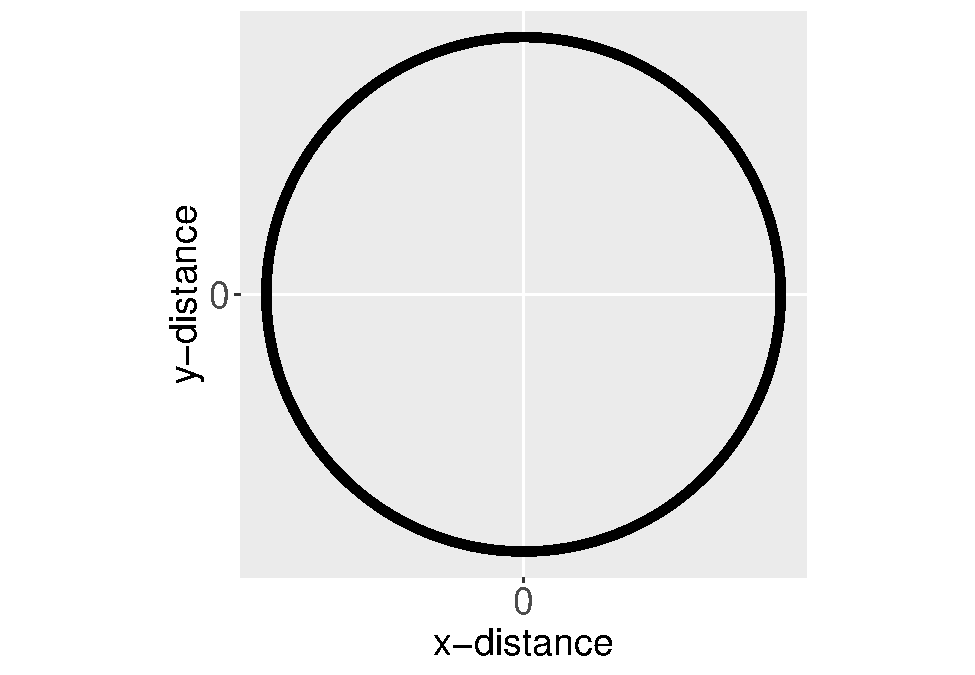
\includegraphics[width=0.49\linewidth]{preprint_files/figure-latex/anisotropy-1} 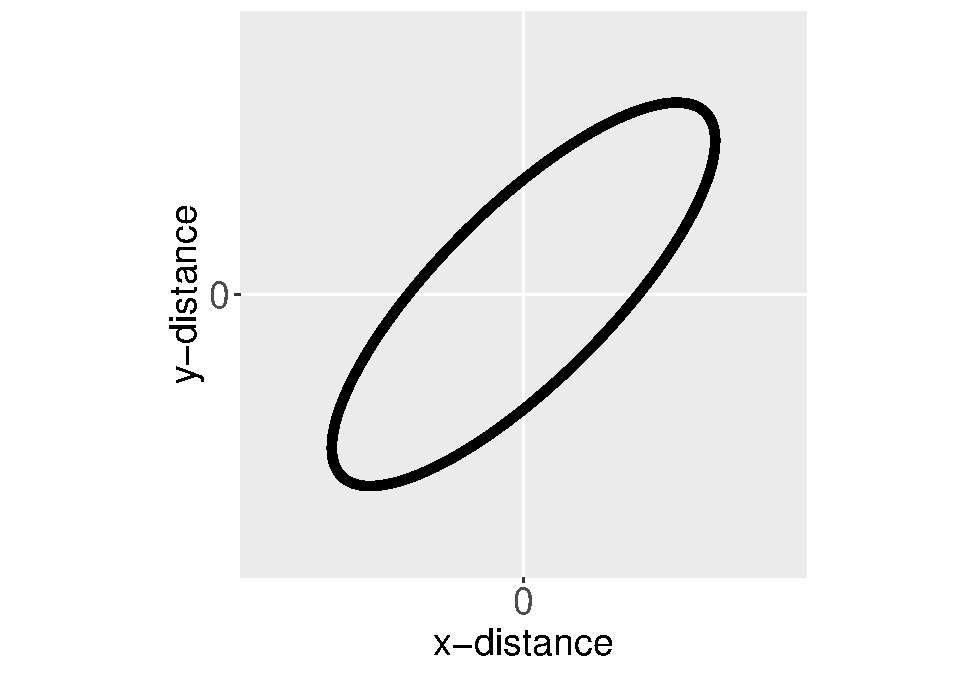
\includegraphics[width=0.49\linewidth]{preprint_files/figure-latex/anisotropy-2} \caption{Ellipses for an isotropic (left) and anisotropic (right) covariance function centered at the origin. The black outline of each ellipse is a level curve of equal correlation.}\label{fig:anisotropy}
\end{figure}

The black outline of each ellipse is a level curve of equal correlation.
The left ellipse (a circle) represents an isotropic covariance function.
The distance at which the correlation between two observations lays on
the level curve is the same in all directions. The right ellipse
represents an anisotropic covariance function. The distance at which the
correlation between two observations lays on the level curve is
different in different directions.

Accounting for anisotropy involves a rotation and scaling of the
x-coordinates and y-coordinates such that the spatial covariance
function that uses these transformed distances is isotropic. We fit a
model with anisotropy by running

\begin{verbatim}
R> spmod_anis <- splm(
+   log_Zn ~ log_dist2road,
+   moss,
+   spcov_type = "exponential",
+   anisotropy = TRUE
+ )
R> summary(spmod_anis)
\end{verbatim}

\begin{verbatim}
Call:
splm(formula = log_Zn ~ log_dist2road, data = moss, spcov_type = "exponential", 
    anisotropy = TRUE)

Residuals:
    Min      1Q  Median      3Q     Max 
-2.5279 -1.2239 -0.7202 -0.1921  1.1659 

Coefficients (fixed):
              Estimate Std. Error z value Pr(>|z|)    
(Intercept)    9.54798    0.22291   42.83   <2e-16 ***
log_dist2road -0.54601    0.01855  -29.44   <2e-16 ***
---
Signif. codes:  0 '***' 0.001 '**' 0.01 '*' 0.05 '.' 0.1 ' ' 1

Pseudo R-squared: 0.7048

Coefficients ( spatial covariance):
       de        ie     range    rotate     scale 
3.561e-01 6.812e-02 8.732e+03 2.435e+00 4.753e-01 
attr(,"class")
[1] "exponential"
\end{verbatim}

The \texttt{rotate} parameter is between zero and \(\pi\) radians and
represents the angle of a clockwise rotation of the ellipse. The
\texttt{scale} parameter is between zero and one and represents the
ratio of the distance between the origin and the edge of the ellipse
along the minor axis to the distance between the origin and the edge of
the ellipse along the major axis. Figure\(~\)\ref{fig:anisotropy_fit}
shows the transformation that turns an anisotropic ellipse into an
isotropic one (i.e., a circle). This transformation requires rotating
the the coordinates clockwise by \texttt{rotate} and then scaling them
the reciprocal of \texttt{scale}. The transformed coordinates are then
used instead of the original coordinates to compute distances and
spatial covariances.

\begin{figure}
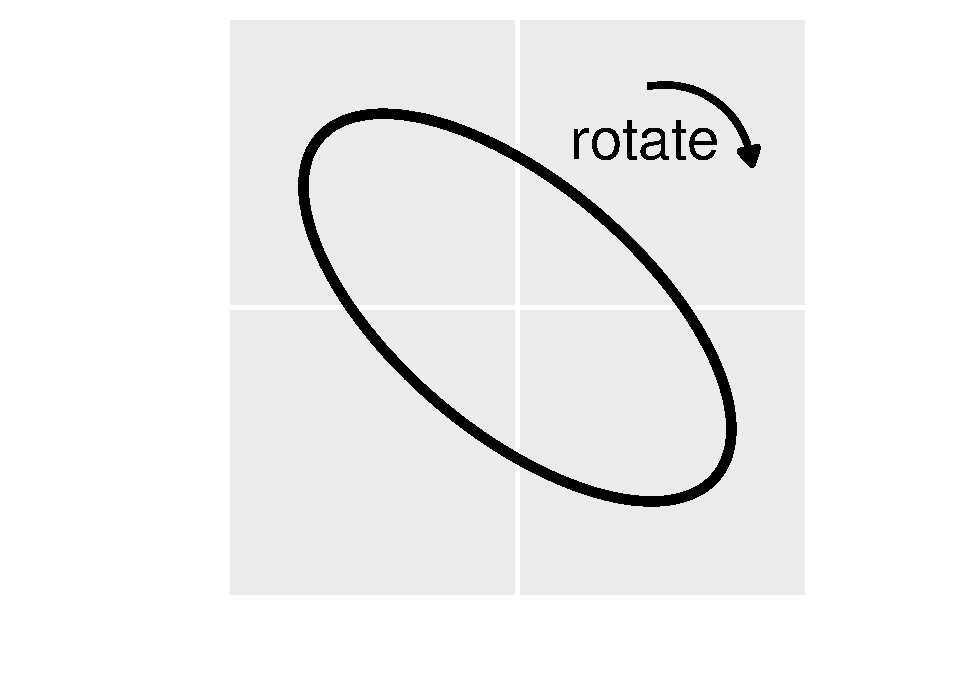
\includegraphics[width=0.33\linewidth]{preprint_files/figure-latex/anisotropy_fit-1} 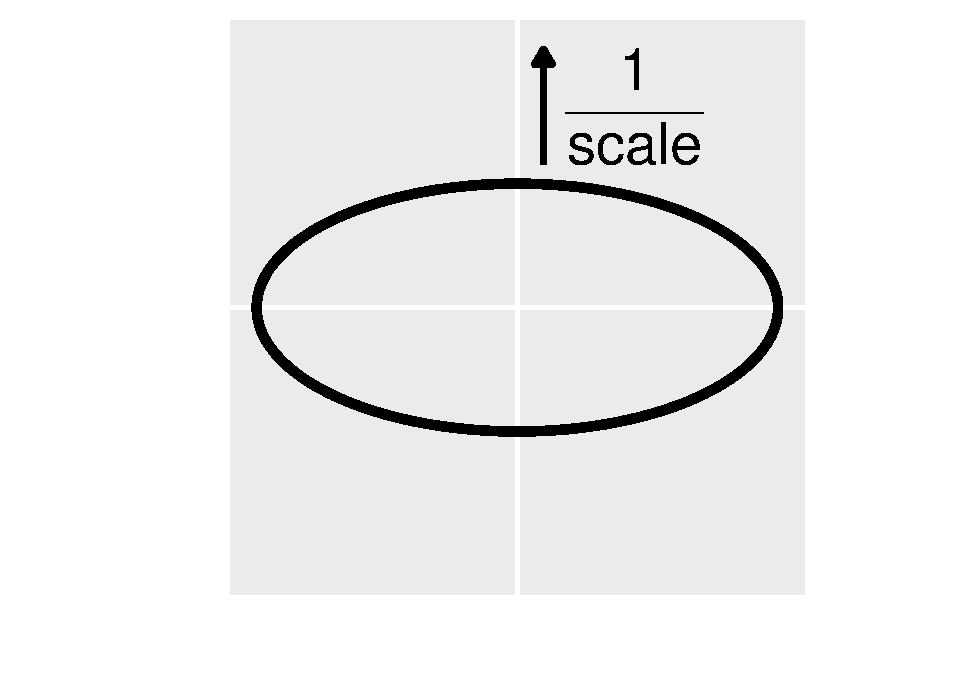
\includegraphics[width=0.33\linewidth]{preprint_files/figure-latex/anisotropy_fit-2} 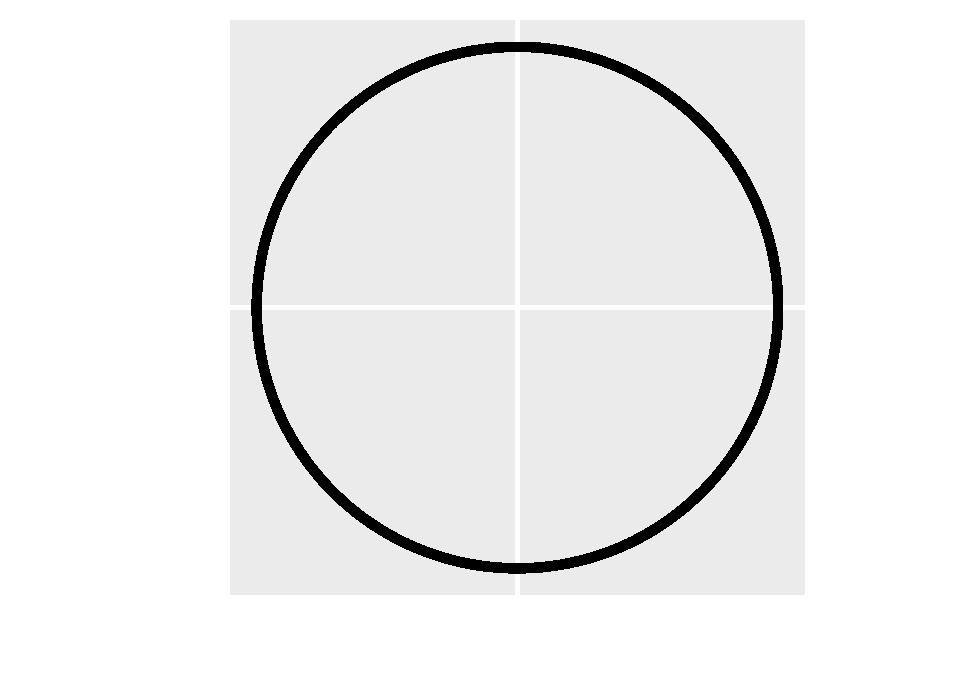
\includegraphics[width=0.33\linewidth]{preprint_files/figure-latex/anisotropy_fit-3} \caption{A visual representation of the anisotropy transformation. In the left figure, the first step is to rotate the anisotropic ellipse clockwise by the \texttt{rotate} parameter. In the middle figure, the second step is to scale the minor axis by the reciprocal of the \texttt{scale} parameter. In the right figure, the anisotropic ellipse has been transformed into an isotropic one (i.e., a circle). The transformed coordinates are then used instead of the original coordinates to compute distances and spatial covariances.}\label{fig:anisotropy_fit}
\end{figure}

Note that specifying an initial value for \texttt{rotate} that is
different from zero, specifying an initial value for \texttt{scale} that
is different from one, or assuming either \texttt{rotate} or
\texttt{scale} are unknown in \texttt{spcov\_initial} will cause
\texttt{splm()} to fit a model with anisotropy (and will override
\texttt{anisotropy\ =\ FALSE}). Estimating anisotropy parameters is only
possible for maximum likelihood and restricted maximum likelihood
estimation, but fixed anisotropy parameters can be accommodated for
semivariogram weighted least squares or semivariogram composite
likelihood estimation. Also note that anisotropy is not relevant for
areal data because the spatial covariance function depends on a
neighborhood structure instead of distances between points.

\hypertarget{sec:sim_data}{%
\subsection{Simulating Spatial Data}\label{sec:sim_data}}

The \texttt{sprnorm()} function is used to simulate normal (Gaussian)
spatial data. To use \texttt{sprnorm()}, the \texttt{spcov\_params()}
function is used to create an \texttt{spcov\_params} object. The
\texttt{spcov\_params()} function requires the spatial covariance type
and and parameter values. We create an \texttt{spcov\_params} object by
running

\begin{verbatim}
R> sim_params <- spcov_params("exponential", de = 5, ie = 1, range = 0.5)
\end{verbatim}

We set a reproducible seed and then simulate data at 3000 random
locations in the unit square using the spatial covariance parameters in
\texttt{sim\_params} by running

\begin{verbatim}
R> set.seed(0)
R> n <- 3000
R> x <- runif(n)
R> y <- runif(n)
R> sim_coords <- tibble::tibble(x, y)
R> sim_resp <- sprnorm(sim_params, data = sim_coords, xcoord = x, ycoord = y)
R> sim_data <- tibble::tibble(sim_coords, sim_resp)
\end{verbatim}

We can visualize the simulated data (Figure\(~\)\ref{fig:sim_preds},
left) by running

\begin{verbatim}
R> ggplot(sim_data, aes(x = x, y = y, color = sim_resp)) +
+   geom_point(size = 1.5) +
+   scale_color_viridis_c(limits = c(-7, 7)) + 
+   theme_gray(base_size = 18)
\end{verbatim}

There is noticeable spatial patterning in the response variable
(\texttt{sim\_resp}). The default mean in \texttt{sprnorm()} is zero for
all observations, though a mean vector can be provided using the
\texttt{mean} argument. The default number of samples generated in
\texttt{sprnorm()} is one, though this is changed using the
\texttt{samples} argument. Because \texttt{dat} is a \texttt{tibble}
(\texttt{data.frame}) and not an \texttt{sf} object, the columns in
\texttt{dat} representing the x-coordinates and y-coordinates must be
provided to \texttt{sprnorm()}.

Note that the output from \texttt{coef(object,\ type\ =\ "spcov")} is a
\texttt{spcov\_params} object. This is useful if one wants to simulate
data given the estimated spatial covariance parameters from a fitted
model. Random effects are incorporated into simulation via the
\texttt{randcov\_params} argument.

\hypertarget{big-data}{%
\subsection{Big Data}\label{big-data}}

The computational cost associated with model fitting is exponential in
the sample size for all estimation methods. For maximum likelihood and
restricted maximum likelihood, the computational cost of estimating
\(\boldsymbol{\theta}\) is cubic. For semivariogram weighted least
squares and semivariogram composite likelihood, the computational cost
of estimating \(\boldsymbol{\theta}\) is quadratic. The computational
cost associated with estimating \(\boldsymbol{\beta}\) and prediction is
cubic in the model-fitting sample size, regardless of estimation method.
Typically samples sizes approaching 10,000 make the computational cost
of model fitting and prediction infeasible, which necessitates the use
of big data methods. \texttt{spmodel} offers big data methods for model
fitting of point-referenced data via the \texttt{local} argument to
\texttt{splm()}, capable of fitting models with hundreds of thousands to
millions of observations rather quickly. Because of the neighborhood
structure of areal data, the big data methods used for point-referenced
data do not apply to areal data. Thus there is no big data method for
areal data or \texttt{local} argument to \texttt{spautor()} and model
fitting sample sizes cannot be too large.

\texttt{spmodel} offers big data methods for prediction of
point-referenced data or areal data via the \texttt{local} argument to
\texttt{predict()}, capable of making predictions at hundreds of
thousands to millions of locations rather quickly. To show how to use
\texttt{spmodel} for big data estimation and prediction, we use the
\texttt{sim\_data} data from Section\(~\)\ref{sec:sim_data}. Because
\texttt{sim\_data} is a \texttt{tibble} (\texttt{data.frame}) and not an
\texttt{sf} object, the column in \texttt{data} representing the
x-coordinates and y-coordinates must be explicitly provided to
\texttt{splm()}. Though the sample sizes used next for model fitting and
prediction are relatively small, the purpose of the following examples
is simply to illustrate the big data approaches.

\hypertarget{model-fitting}{%
\subsubsection{Model-fitting}\label{model-fitting}}

\texttt{spmodel} uses a ``local indexing'' approximation for big data
model fitting of point-referenced data. Observations are first assigned
an index. Then for the purposes of model fitting, observations with
different indexes are assumed uncorrelated. This approach has some
connections to composite likelihood and to the partition factors
discussed earlier.

The \texttt{local} argument to \texttt{splm()} controls the big data
options. \texttt{local} is a list with several arguments. The arguments
to the \texttt{local} list control the method used to assign the
indexes, the number of observations with the same index, the number of
unique indexes, variance adjustments to the covariance matrix of
\(\hat{\boldsymbol{\beta}}\), whether or not to use parallel processing,
and if parallel processing is used, the number of cores.

The simplest way to accommodate big data is to set \texttt{local} to
\texttt{TRUE}. This is shorthand for
\texttt{local\ =\ list(method\ =\ "random",\ size\ =\ 50,\ var\_adjust\ =\ "theoretical",\ parallel\ =\ FALSE)},
which creates groups with approximately 50 observations each using a
random assignment of groups to indexes, uses the theoretically-correct
variance adjustment, and does not use parallel processing.

\begin{verbatim}
R> local1 <- splm(sim_resp ~ 1, sim_data, spcov_type = "exponential", 
+                xcoord = x, ycoord = y, local = TRUE)
R> summary(local1)
\end{verbatim}

\begin{verbatim}
Call:
splm(formula = sim_resp ~ 1, data = sim_data, spcov_type = "exponential", 
    xcoord = x, ycoord = y, local = TRUE)

Residuals:
    Min      1Q  Median      3Q     Max 
-5.0356 -1.3514 -0.1468  1.2842  6.5381 

Coefficients (fixed):
            Estimate Std. Error z value Pr(>|z|)
(Intercept)   -1.021      0.699   -1.46    0.144

Coefficients ( spatial covariance):
    de     ie  range 
2.8724 0.9735 0.2644 
\end{verbatim}

Instead of using \texttt{local\ =\ TRUE}, we can explicitly set
\texttt{local}. For example, we fit a model using using k-means
clustering (MacQueen and others 1967) on the x-coordinates and
y-coordinates to create 60 groups (clusters), the pooled variance
adjustment, and parallel processing with two cores by running

\begin{verbatim}
R> local2_list <- list(method = "kmeans", groups = 60, var_adjust = "pooled",
+                     parallel = TRUE, ncores = 2)
R> local2 <- splm(sim_resp ~ 1, sim_data, spcov_type = "exponential", 
+                xcoord = x, ycoord = y, local = local2_list)
R> summary(local2)
\end{verbatim}

\begin{verbatim}
Call:
splm(formula = sim_resp ~ 1, data = sim_data, spcov_type = "exponential", 
    xcoord = x, ycoord = y, local = local2_list)

Residuals:
     Min       1Q   Median       3Q      Max 
-4.98801 -1.30386 -0.09927  1.33176  6.58567 

Coefficients (fixed):
            Estimate Std. Error z value Pr(>|z|)    
(Intercept)  -1.0683     0.1759  -6.073 1.25e-09 ***
---
Signif. codes:  0 '***' 0.001 '**' 0.01 '*' 0.05 '.' 0.1 ' ' 1

Coefficients ( spatial covariance):
    de     ie  range 
2.5434 0.9907 0.2312 
\end{verbatim}

We can use \texttt{loocv()} to evaluate model fit. Note that
\texttt{loocv()} has big data options that are passed to
\texttt{predict()}, which we discuss in Section\(~\)\ref{sec:predict}.

\begin{verbatim}
R> loocv(local1, local = list(method = "distance", parallel = TRUE, ncores = 2))
\end{verbatim}

\begin{verbatim}
[1] 1.243062
\end{verbatim}

\begin{verbatim}
R> loocv(local2, local = list(method = "distance", parallel = TRUE, ncores = 2))
\end{verbatim}

\begin{verbatim}
[1] 1.242925
\end{verbatim}

Likelihood-based statistics like \texttt{AIC()}, \texttt{AICc()},
\texttt{logLik()}, and \texttt{deviance()} should not be used to compare
a model fit with a big data approximation to a model fit without a big
data approximation, as the two approaches maximize different
likelihoods.

\hypertarget{sec:predict}{%
\subsubsection{Prediction}\label{sec:predict}}

For point-referenced data, \texttt{spmodel} uses a ``local
neighborhood'' approximation for big data prediction. Each prediction is
computed using a subset of the observed data instead of all the observed
data. Before further discussing big data prediction, we simulate 1000
locations in the unit square requiring prediction:

\begin{verbatim}
R> n_pred <- 1000
R> x <- runif(n_pred)
R> y <- runif(n_pred)
R> sim_preds <- tibble::tibble(x = x, y = y)
\end{verbatim}

The \texttt{local} argument to \texttt{predict()} controls the big data
options. \texttt{local} is a list with several arguments. The arguments
to the \texttt{local} list control the method used to subset the
observed data, the number of observations in each subset, whether or not
to use parallel processing, and if parallel processing is used, the
number of cores.

The simplest way to accommodate big data prediction is to set
\texttt{local} to \texttt{TRUE}. This is shorthand for
\texttt{local\ =\ list(method\ =\ "covariance",\ size\ =\ 50,\ parallel\ =\ FALSE)},
which implies that uniquely for each location requiring prediction, only
the 50 observations in the data most correlated with it are used in the
computation and parallel processing is not used. Using the
\texttt{local1} fitted model, we store these predictions as a variable
called \texttt{preds} in the \texttt{sim\_preds} data by running

\begin{verbatim}
R> sim_preds$preds <- predict(local1, newdata = sim_preds, local = TRUE)
\end{verbatim}

The predictions are visualized (Figure\(~\)\ref{fig:sim_preds}, right)
by running

\begin{verbatim}
R> ggplot(sim_preds, aes(x = x, y = y, color = preds)) +
+   geom_point(size = 1.5) +
+   scale_color_viridis_c(limits = c(-7, 7)) + 
+   theme_gray(base_size = 18)
\end{verbatim}

They display a similar pattern as the observed data.

\begin{figure}

{\centering 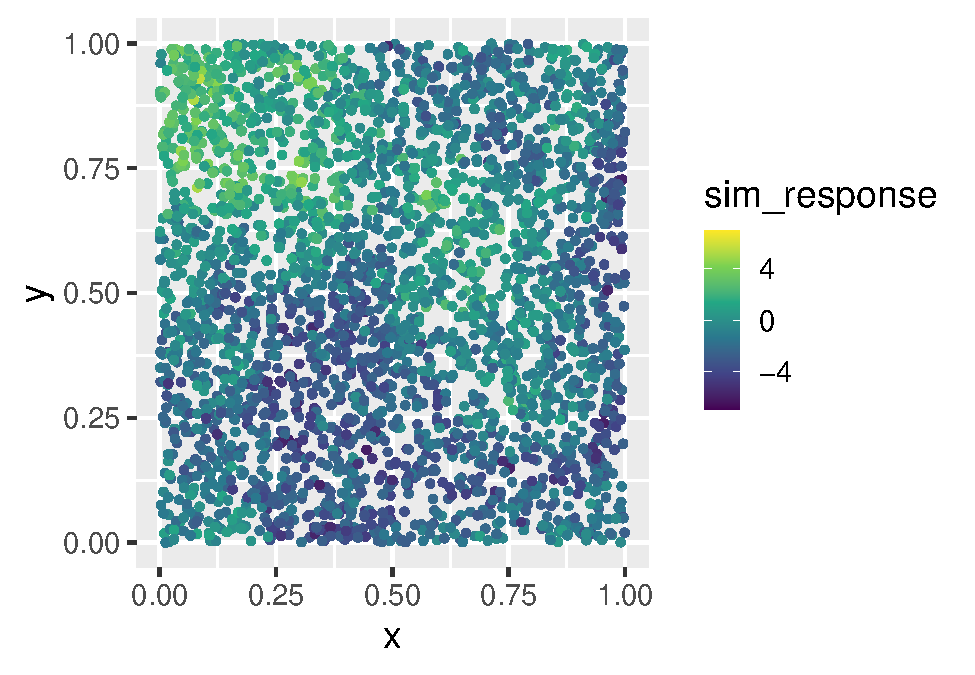
\includegraphics[width=0.49\linewidth]{preprint_files/figure-latex/sim_preds-1} 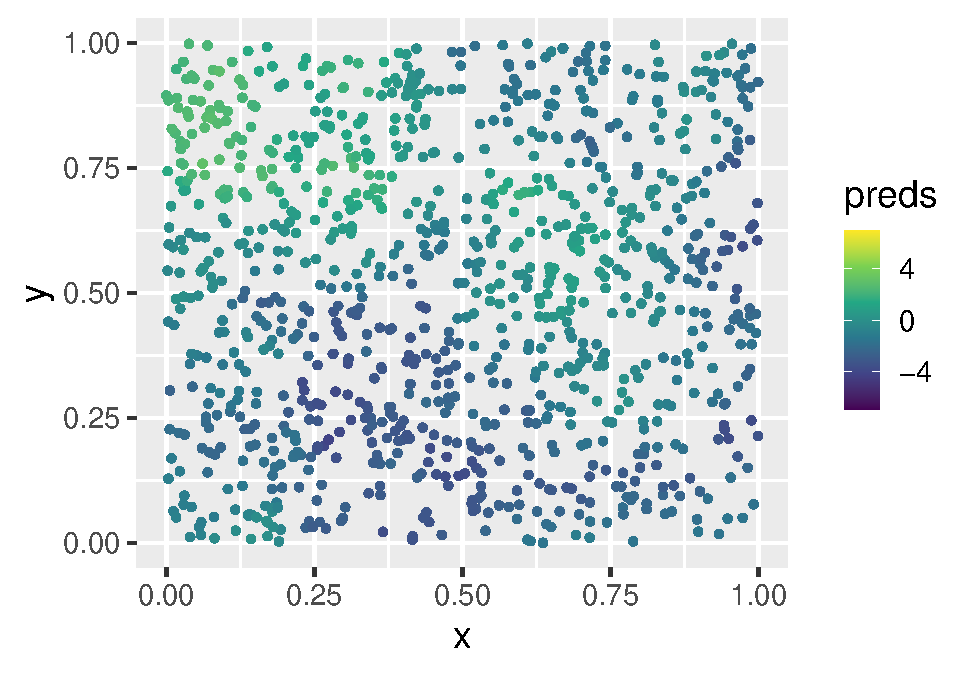
\includegraphics[width=0.49\linewidth]{preprint_files/figure-latex/sim_preds-2} 

}

\caption{Observed data and big data predictions at unobserved locations. In the left figure, spatial data are simulated in the unit square. A spatial linear model is fit using the default big data approximation for model-fitting. In the right figure, predictions are made using the fitted model and the default big data approximation for prediction.}\label{fig:sim_preds}
\end{figure}

Instead of using \texttt{local\ =\ TRUE}, we can explicitly set
\texttt{local}. For example, we make predictions using the distance
method, subsets of 30 observations, and parallel processing with 2 cores
by running

\begin{verbatim}
R> pred_list <- list(method = "distance", size = 30, parallel = TRUE, ncores = 2)
R> predict(local1, newdata = sim_preds, local = pred_list)
\end{verbatim}

For areal data, no local neighborhood approximation exists because of
the data's underlying neighborhood structure. Thus all of the data must
be used to compute predictions and by consequence, \texttt{method} and
\texttt{distance} are not components of the \texttt{local} list. The
only components of the \texttt{local} list for areal data are
\texttt{parallel} and \texttt{ncores}:

\begin{verbatim}
R> predict(sealmod, local = list(parallel = TRUE, ncores = 2))
\end{verbatim}

\hypertarget{sec:discussion}{%
\section{Discussion}\label{sec:discussion}}

\texttt{spmodel} is a novel, relevant contribution used to fit,
summarize, and predict for a variety of spatial statistical models.
Spatial linear models for point-referenced data (i.e., geostatistical
models) are fit using the \texttt{splm()} function. Spatial linear
models for areal data (i.e., spatial autoregressive models) are fit
using the \texttt{spautor()} function. Several model-fit statistics and
diagnostics are available. The broom functions \texttt{tidy()} and
\texttt{glance()} are used to tidy and glance at a fitted model. The
broom function \texttt{augment()} is used to augment \texttt{data} with
model diagnostics and augment \texttt{newdata} with predictions. Several
advanced features are available to accommodate fixed covariance
parameter values, random effects, partition factors, anisotropy,
simulated data, and big data approximations for model fitting and
prediction.

We appreciate feedback from users regarding \texttt{spmodel}. To learn
more about how to provide feedback or contribute to \texttt{spmodel},
please visit our GitHub repository at
\url{https://github.com/USEPA/spmodel}. Possible \texttt{spmodel}
extensions including machine learning methods, generalized linear mixed
models, and Bayesian models.

\hypertarget{references}{%
\section*{References}\label{references}}
\addcontentsline{toc}{section}{References}

\hypertarget{refs}{}
\begin{CSLReferences}{1}{0}
\leavevmode\hypertarget{ref-bates2015lme4}{}%
Bates, Douglas, Martin Mächler, Ben Bolker, and Steve Walker. 2015.
{``Fitting Linear Mixed-Effects Models Using {lme4}.''} \emph{Journal of
Statistical Software} 67 (1): 1--48.
\url{https://doi.org/10.18637/jss.v067.i01}.

\leavevmode\hypertarget{ref-cook1982residuals}{}%
Cook, R Dennis, and Sanford Weisberg. 1982. \emph{Residuals and
Influence in Regression}. New York: Chapman; Hall.

\leavevmode\hypertarget{ref-cressie1985fitting}{}%
Cressie, Noel. 1985. {``Fitting Variogram Models by Weighted Least
Squares.''} \emph{Journal of the International Association for
Mathematical Geology} 17 (5): 563--86.

\leavevmode\hypertarget{ref-curriero1999composite}{}%
Curriero, Frank C, and Subhash Lele. 1999. {``A Composite Likelihood
Approach to Semivariogram Estimation.''} \emph{Journal of Agricultural,
Biological, and Environmental Statistics}, 9--28.

\leavevmode\hypertarget{ref-nychka2021fields}{}%
Douglas Nychka, Reinhard Furrer, John Paige, and Stephan Sain. 2021.
{``Fields: Tools for Spatial Data.''} Boulder, CO, USA: University
Corporation for Atmospheric Research.
\url{https://github.com/dnychka/fieldsRPackage}.

\leavevmode\hypertarget{ref-dumelle2022comparison}{}%
Dumelle, Michael, Matt Higham, Jay M Ver Hoef, Anthony R Olsen, and Lisa
Madsen. 2022. {``A Comparison of Design-Based and Model-Based Approaches
for Finite Population Spatial Sampling and Inference.''} \emph{Methods
in Ecology and Evolution}.

\leavevmode\hypertarget{ref-dumelle2022spsurvey}{}%
Dumelle, Michael, Thomas M Kincaid, Anthony R Olsen, and Marc H Weber.
2022. \emph{Spsurvey: Spatial Sampling Design and Analysis}.
\url{https://CRAN.R-project.org/package=spsurvey}.

\leavevmode\hypertarget{ref-finley2007spbayes}{}%
Finley, Andrew O., Sudipto Banerjee, and Bradley P. Carlin. 2007.
{``{spBayes}: An {R} Package for Univariate and Multivariate
Hierarchical Point-Referenced Spatial Models.''} \emph{Journal of
Statistical Software} 19 (4): 1--24.
\url{https://www.jstatsoft.org/article/view/v019i04}.

\leavevmode\hypertarget{ref-finley2002spnngp}{}%
Finley, Andrew O., Abhirup Datta, and Sudipto Banerjee. 2022.
{``{spNNGP} {R} Package for Nearest Neighbor {G}aussian Process
Models.''} \emph{Journal of Statistical Software} 103 (5): 1--40.
\url{https://doi.org/10.18637/jss.v103.i05}.

\leavevmode\hypertarget{ref-guiness2021gpgp}{}%
Guiness, Joseph, Matthias Katzfuss, and Youssef Fahmy. 2021. \emph{GpGp:
Fast Gaussian Process Computation Using Vecchia's Approximation}.
\url{https://CRAN.R-project.org/package=GpGp}.

\leavevmode\hypertarget{ref-harville1977maximum}{}%
Harville, David A. 1977. {``Maximum Likelihood Approaches to Variance
Component Estimation and to Related Problems.''} \emph{Journal of the
American Statistical Association} 72 (358): 320--38.

\leavevmode\hypertarget{ref-hoeting2006model}{}%
Hoeting, Jennifer A, Richard A Davis, Andrew A Merton, and Sandra E
Thompson. 2006. {``Model Selection for Geostatistical Models.''}
\emph{Ecological Applications} 16 (1): 87--98.

\leavevmode\hypertarget{ref-lee2013carbayes}{}%
Lee, Duncan. 2013. {``{CARBayes}: An {R} Package for {B}ayesian Spatial
Modeling with Conditional Autoregressive Priors.''} \emph{Journal of
Statistical Software} 55 (13): 1--24.
\url{https://www.jstatsoft.org/htaccess.php?volume=55\&type=i\&issue=13}.

\leavevmode\hypertarget{ref-macqueen1967some}{}%
MacQueen, James, and others. 1967. {``Some Methods for Classification
and Analysis of Multivariate Observations.''} In \emph{Proceedings of
the Fifth Berkeley Symposium on Mathematical Statistics and
Probability}, 1:281--97. 14. Oakland, CA, USA.

\leavevmode\hypertarget{ref-montgomery2021introduction}{}%
Montgomery, Douglas C, Elizabeth A Peck, and G Geoffrey Vining. 2021.
\emph{Introduction to Linear Regression Analysis}. John Wiley \& Sons.

\leavevmode\hypertarget{ref-nychka2016latticekrig}{}%
Nychka, Douglas, Dorit Hammerling, Stephan Sain, and Nathan Lenssen.
2016. {``LatticeKrig: Multiresolution Kriging Based on Markov Random
Fields.''} Boulder, CO, USA: University Corporation for Atmospheric
Research. \url{https://doi.org/10.5065/D6HD7T1R}.

\leavevmode\hypertarget{ref-patterson1971recovery}{}%
Patterson, H Desmond, and Robin Thompson. 1971. {``Recovery of
Inter-Block Information When Block Sizes Are Unequal.''}
\emph{Biometrika} 58 (3): 545--54.

\leavevmode\hypertarget{ref-pebesma2018sf}{}%
Pebesma, Edzer. 2018. {``{Simple Features for R: Standardized Support
for Spatial Vector Data}.''} \emph{{The R Journal}} 10 (1): 439--46.
\url{https://doi.org/10.32614/RJ-2018-009}.

\leavevmode\hypertarget{ref-pebesma2004gstat}{}%
Pebesma, Edzer J. 2004. {``Multivariable Geostatistics in {S}: The Gstat
Package.''} \emph{Computers \& Geosciences} 30: 683--91.

\leavevmode\hypertarget{ref-pinheiro2006mixed}{}%
Pinheiro, José, and Douglas Bates. 2006. \emph{Mixed-Effects Models in s
and s-PLUS}. Springer science \& business media.

\leavevmode\hypertarget{ref-ribiero2022geoR}{}%
Ribeiro Jr, Paulo Justiniano, Peter Diggle, Ole Christensen, Martin
Schlather, Roger Bivand, and Brian Ripley. 2022. \emph{geoR: Analysis of
Geostatistical Data}. \url{https://CRAN.R-project.org/package=geoR}.

\leavevmode\hypertarget{ref-robinson2021broom}{}%
Robinson, David, Alex Hayes, and Simon Couch. 2021. \emph{Broom: Convert
Statistical Objects into Tidy Tibbles}.
\url{https://CRAN.R-project.org/package=broom}.

\leavevmode\hypertarget{ref-ronnegard2010hglm}{}%
Ronnegard, Lars, Xia Shen, and Moudud Alam. 2010. {``Hglm: A Package for
Fitting Hierarchical Generalized Linear Models.''} \emph{The R Journal}
2 (2): 20--28.
\url{https://journal.r-project.org/archive/2010-2/RJournal_2010-2_Roennegaard~et~al.pdf}.

\leavevmode\hypertarget{ref-tobler1970computer}{}%
Tobler, Waldo R. 1970. {``A Computer Movie Simulating Urban Growth in
the Detroit Region.''} \emph{Economic Geography} 46 (sup1): 234--40.

\leavevmode\hypertarget{ref-venables2002S}{}%
Venables, W. N., and B. D. Ripley. 2002. \emph{Modern Applied Statistics
with s}. Fourth. New York: Springer.
\url{https://www.stats.ox.ac.uk/pub/MASS4/}.

\leavevmode\hypertarget{ref-wickham2016ggplot2}{}%
Wickham, Hadley. 2016. \emph{Ggplot2: Elegant Graphics for Data
Analysis}. Springer-Verlag New York.
\url{https://ggplot2.tidyverse.org}.

\leavevmode\hypertarget{ref-wolfinger1994computing}{}%
Wolfinger, Russ, Randy Tobias, and John Sall. 1994. {``Computing
Gaussian Likelihoods and Their Derivatives for General Linear Mixed
Models.''} \emph{SIAM Journal on Scientific Computing} 15 (6):
1294--1310.

\leavevmode\hypertarget{ref-zammitmangion2021FRK}{}%
Zammit-Mangion, Andrew, and Noel Cressie. 2021. {``FRK: An r Package for
Spatial and Spatio-Temporal Prediction with Large Datasets.''}
\emph{Journal of Statistical Software} 98 (4): 1--48.

\end{CSLReferences}

\newpage

\hypertarget{appendices}{%
\section*{Appendices}\label{appendices}}
\addcontentsline{toc}{section}{Appendices}

\renewcommand{\thesubsection}{\Alph{subsection}}

\hypertarget{app:caribou}{%
\subsection{\texorpdfstring{An Additional Example Using
\texttt{caribou}}{An Additional Example Using caribou}}\label{app:caribou}}

The \texttt{caribou} data are observed on an equally spaced lattice and
can be analyzed as point-referenced or areal data. We view the first few
rows of \texttt{caribou} by running

\begin{verbatim}
R> caribou
\end{verbatim}

\begin{verbatim}
# A tibble: 30 x 5
   water tarp      z     x     y
   <fct> <fct> <dbl> <dbl> <dbl>
 1 Y     clear  2.42     1     6
 2 Y     shade  2.44     2     6
 3 Y     none   1.81     3     6
 4 N     clear  1.97     4     6
 5 N     shade  2.38     5     6
 6 Y     none   2.22     1     5
 7 N     clear  2.10     2     5
 8 Y     clear  1.80     3     5
 9 Y     shade  1.96     4     5
10 Y     none   2.10     5     5
# ... with 20 more rows
\end{verbatim}

First we analyze \texttt{caribou} as point-referenced data. Because
\texttt{caribou} is not an \texttt{sf} object, we must provide the
columns in \texttt{caribou} that represent the x-coordinates and
y-coordinates. We fit a spatial linear model regressing nitrogen
percentage (\texttt{z}) on water presence (\texttt{water}) and tarp
cover (\texttt{tarp}) by running

\begin{verbatim}
R> cariboumod <- splm(z ~ water + tarp, data = caribou,
+                    spcov_type = "exponential", xcoord = x, ycoord = y)
\end{verbatim}

An analysis of variance can be conducted to assess the overall impact of
the \texttt{tarp} variable, which has three levels (clear, shade, and
none), and the \texttt{water} variable, which has two levels (water and
no water). We perform an analysis of variance and tidy the results by
running

\begin{verbatim}
R> tidy(anova(cariboumod))
\end{verbatim}

\begin{verbatim}
# A tibble: 3 x 4
  effects        df statistic  p.value
  <chr>       <int>     <dbl>    <dbl>
1 (Intercept)     1     43.5  4.33e-11
2 water           1      1.66 1.98e- 1
3 tarp            2     15.4  4.51e- 4
\end{verbatim}

There is significant evidence that at least one tarp cover impacts
nitrogen. Note that, like in \texttt{summary()}, these p-values are
associated with an asymptotic hypothesis test (here, an asymptotic
Chi-squared test).

Next we analyze \texttt{caribou} as areal data. Because \texttt{caribou}
is not an \texttt{sf} object, we must create a weights matrix. We define
two observations as neighbors if they are adjacent (directly east, west,
north, or south) to one another. Two observations in \texttt{caribou}
are adjacent if the distance between them equals one (recall that
observations are not neighbors with themselves):

\begin{verbatim}
R> coords <- cbind(caribou$x, caribou$y)
R> dists <- as.matrix(dist(coords))
R> W <- dists == 1
\end{verbatim}

Currently, \texttt{W} is a logical matrix with \texttt{TRUE}s and
\texttt{FALSE}s. We coerce it to a numeric matrix by running

\begin{verbatim}
R> W <- W * 1
\end{verbatim}

The \(ij\)th value in \texttt{W} is \texttt{1} if the observation in the
\(i\)th row is neighbors with the observation in the \(j\)th row and
\texttt{0} otherwise. We fit a spatial autoregressive model regressing
the nitrogen percentage (\texttt{z}) on water presence (\texttt{water})
and tarp cover (\texttt{tarp}) by running

\begin{verbatim}
R> cariboumod <- spautor(z ~ water + tarp, data = caribou,
+                       spcov_type = "car", W = W)
\end{verbatim}

We perform an analysis of variance and tidy the results by running

\begin{verbatim}
R> tidy(anova(cariboumod))
\end{verbatim}

\begin{verbatim}
# A tibble: 3 x 4
  effects        df statistic   p.value
  <chr>       <int>     <dbl>     <dbl>
1 (Intercept)     1    714.   2.36e-157
2 water           1      1.82 1.77e-  1
3 tarp            2     15.1  5.17e-  4
\end{verbatim}

There is significant evidence that at least one tarp cover impacts
nitrogen. Note that, like in \texttt{summary()}, these p-values are
associated with an asymptotic hypothesis test (here, an asymptotic
Chi-squared test).

\hypertarget{app:rand}{%
\subsection{Random Effect Syntax}\label{app:rand}}

A couple of common ways to specify random effects in the \texttt{random}
argument to \texttt{splm()} or \texttt{spautor()} include:

\begin{itemize}
\tightlist
\item
  \texttt{\textasciitilde{}\ (1\ \textbar{}\ group)} : Random intercepts
  for each level of \texttt{group}. \texttt{\textasciitilde{}\ group} is
  shorthand for \texttt{\textasciitilde{}\ (1\ \textbar{}\ group)}.
\item
  \texttt{\textasciitilde{}\ (var\ \textbar{}\ group)}: Random
  intercepts for each level of \texttt{group} and random slopes that
  depend on the variable \texttt{var} for each level of \texttt{group}.
\end{itemize}

Some additional syntax for more complicated random effects structures
include:

\begin{itemize}
\tightlist
\item
  \texttt{\textasciitilde{}\ (var\ -\ 1\ \textbar{}\ group)}: Random
  slopes (without intercepts) that depend on the variable \texttt{var}
  for each level of \texttt{group}.
\item
  \texttt{\textasciitilde{}\ (1\ \textbar{}\ group:subgroup)}: Random
  intercepts for each combination of levels in \texttt{group} and levels
  in \texttt{subgroup}. \texttt{\textasciitilde{}\ group:subgroup} is
  shorthand for
  \texttt{\textasciitilde{}\ (1\ \textbar{}\ group:subgroup)}.
\item
  \texttt{\textasciitilde{}\ (var\ \textbar{}\ group:subgroup)}: Random
  intercepts for each combination of levels in \texttt{group} and levels
  in \texttt{subgroup} and random slopes that depend on the variable
  \texttt{var} for each combination of levels in \texttt{group} and
  levels in \texttt{subgroup}.
\item
  \texttt{\textasciitilde{}\ (var\ -\ 1\ \textbar{}\ group:subgroup)}:
  Random slopes (without intercepts) that depend on the variable
  \texttt{var} for each combination of levels in \texttt{group} and
  levels in \texttt{subgroup}.
\item
  \texttt{\textasciitilde{}\ (1\ \textbar{}\ group/subgroup)}: Shorthand
  for
  \texttt{\textasciitilde{}\ (1\ \textbar{}\ group)\ +\ (1\ \textbar{}\ group:subgroup)}.
  Commonly, the \texttt{group/subgroup} notation implies
  \texttt{subgroup} is nested within \texttt{group}.
\item
  \texttt{\textasciitilde{}\ (var\ \textbar{}\ group/subgroup)}:
  Shorthand for
  \texttt{\textasciitilde{}\ (var\ \textbar{}\ group)\ +\ (var\ \textbar{}\ group:subgroup)}.
  Commonly, the \texttt{group/subgroup} notation implies
  \texttt{subgroup} is nested within \texttt{group}.
\item
  \texttt{\textasciitilde{}\ (var\ -\ 1\ \textbar{}\ group/subgroup)}:
  Shorthand for
  \texttt{\textasciitilde{}\ (var\ -\ 1\ \textbar{}\ group)\ +\ (var\ -\ 1\ \textbar{}\ group:subgroup)}.
  Commonly, the \texttt{group/subgroup} notation implies
  \texttt{subgroup} is nested within \texttt{group}.
\end{itemize}

Distinct random effects terms are separated in \texttt{random} by
\texttt{+}. Each term must be wrapped in parentheses. For example, to
incorporate random intercepts for \texttt{group} and \texttt{subgroup},
\texttt{random} looks like
\texttt{\textasciitilde{}\ (1\ \textbar{}\ group)\ +\ (1\ \textbar{}\ subgroup)}.
For random intercepts, recall that \texttt{\textasciitilde{}\ group} is
shorthand for \texttt{\textasciitilde{}\ (1\ \textbar{}\ group)}. Thus,
an equivalent representation of
\texttt{\textasciitilde{}\ (1\ \textbar{}\ group)\ +\ (1\ \textbar{}\ subgroup)}
is \texttt{\textasciitilde{}\ group\ +\ subgroup}. Note that for both
random intercepts and random slopes, the variable on the right-hand side
of \texttt{\textbar{}} (i.e., \texttt{group}, \texttt{subgroup},
\texttt{group:subgroup}) must be a factor (or character) variable.

\bibliographystyle{natbib}
\bibliography{references.bib}


\end{document}
